\documentclass[a4paper, oneside]{discothesis}

\usepackage[utf8]{inputenc}
\usepackage[T1]{fontenc}
\usepackage{algpseudocode}
\usepackage{algorithm}
\usepackage{mathtools}
\usepackage{pgfplots}
\usepackage{subcaption}
\usepackage{tikz}
\usepackage{hyperref}
\usepackage{minted}
\usepackage{commath}
\usetikzlibrary{arrows.meta}
\usetikzlibrary{pgfplots.groupplots}

\def\sectionautorefname{Section}
\def\subsectionautorefname{Subsection}
\def\paragraphautorefname{Paragraph}
\def\chapterautorefname{Chapter}
\def\figureautorefname{Figure}

\title{Arvy Heuristics for \\Distributed Mutual Exclusion}
\thesistype{Bachelor's Thesis}

\author{Silvan Mosberger}
\email{msilvan@student.ethz.ch}

\institute{Distributed Computing Group \\[2pt]
Computer Engineering and Networks Laboratory \\[2pt]
ETH Zürich}

\supervisors{Pankaj Khanchandani, András Papp\\[2pt] Prof.\ Dr.\ Roger Wattenhofer}

\keywords{Arrow, Ivy, distributed directory protocol, distributed mutual exclusion}
\categories{Network algorithms}

\date{\today}

\begin{document}

\frontmatter
\maketitle

\cleardoublepage

\begin{acknowledgements}
I thank my advisors Pankaj and András for the weekly discussions, which helped greatly in guiding the direction of this work and developing new ideas. They helped me focus on the important bits without getting distracted too much. This is in contrast to all the cats wanting to sit on my lap or desk all the time, which I'm still grateful for however. I also thank my colleagues for giving me company when I needed it and being good friends.
\end{acknowledgements}


\begin{abstract}
In this thesis we look at different heuristics for the Arvy-class of algorithms for solving the distributed mutual exclusion problem, focusing on sequential requests. This includes the previously known algorithms Arrow and Ivy but many new ones as well. We will see that Arrow with a star tree is one of the best solutions in many cases. However we show that a new heuristic based on Ivy in a nested clique-like graph can have better performance still. In addition another new heuristic based on measuring request probabilities allows for better performance with adversarial requests. To evaluate the running time of Arvy heuristics, a flexible Haskell library was developed whose types guarantee correctness at compile time.
\end{abstract}

\tableofcontents

\mainmatter

\chapter{Introduction}

Often in computing a single resource is shared between multiple components, where only one of them may access it at a time. Components can request the resource at any time, after which they should receive it eventually. In a distributed setting an algorithm to solve this is called a distributed mutual exclusion algorithm or distributed directory protocol. A trivial solution is to dedicate a single node to be the center where all requests for the resource should go, with the disadvantage of a lot of traffic and contention for many concurrent requests. Better solutions to this problem include the spanning-tree-based Arrow (also known as Raymond's algorithm) and Ivy protocols, introduced in \cite{Ray} and \cite{Ivy} respectively. Both of these algorithms can be generalized to the Arvy-class of algorithms, introduced in \cite{Arvy}, which allows for a wide range of different heuristics to be used for determining its behavior, while still guaranteeing correctness. There also exist other kinds of algorithms to solve this problem based on message broadcasting or quorums.

In this thesis we come up with new Arvy heuristics and measure their empirical performance in a simulation of sequential requests.

\section{Related Work}

Arvy was introduced in \cite{Arvy} where it was also shown to be correct in asynchronous networks with concurrent requests in arbitrary networks. In \cite{Kuhn} it was shown that Arrow is $\mathcal{O}(\log D)$ competitive where $D$ is the diameter of the spanning tree it operates on. 

\TODO{Ivy Fibonacci tree}

\newpage
\section{Model}\label{model}

We consider a complete graph $G=(V,E)$ with $n$ vertices and $\binom{n}{2}$ edges.

\paragraph{Metric Costs} Each edge has a cost/distance $c : E \rightarrow \mathbb{R}^+$ associated with it, representing the amount of time it takes a message to traverse it. This function forms a metric space:
\begin{itemize}
\item The cost from a node to itself is zero: $\forall v:c(v, v)=0$
\item Costs between different nodes are positive: $\forall u,v : u\neq v\Rightarrow c(u,v)>0$
\item Costs are the same in both directions: $\forall u,v : c(u,v)=c(v,u)$
\item The triangle inequality holds: $\forall u,v,w : c(u,w)\leq c(u,v)+c(v,w)$
\end{itemize}

As a reasonable constraint, a node $v$ can only query costs from itself to other nodes, so it only has access to the $n$ cost values $\{c(v, u)\;|\;u\in V\}$. In a realistic scenario it's these costs that can be obtained and updated by doing regular pings to other nodes. While we don't consider changing costs in our model, there's no inherent reason the heuristic we describe can't work in such cases.

\paragraph{Instantaneous Computations} In addition, every node can be considered a machine with the ability to execute arbitrary effectful code such as reading/writing state or generating randomness. We model execution to be instantaneous such that no time passes for computations in nodes. Therefore traversing graph edges are the only place to spend time on.

\paragraph{Sequential Requests} A major simplification we make is that nodes can only request the token sequentially. So only after the token has reached the requesting node, another node can make a request for it. Therefore requests can be represented as a series $R=\{r_1,r_2,\dots\},r_i\in V$ where $r_i$ encodes the $i$-th request originating from node $r_i$. While this series could go on forever, we let it be finite such that we can reason about it's total execution time.

\paragraph{Request Paths} In the type of algorithms we'll look at, when the $i$-th request gets made by node $r_i$, the request travels along some path $A^{(i)}=\{a^{(i)}_0,a^{(i)}_1,\dots,a^{(i)}_{l_i}\}$ with $l_i=|A^{(i)}|-1$ being the index of the last node and also the number of messages that are being sent. $a^{(i)}_0=r_i$ is the node making the request and the $a^{(i)}_{l_i}$ is the node currently holding the token. After the request was sent along this path, the token is then sent directly from $a^{(i)}_{l_i}$ to $a^{(i)}_0$ to satisfy the request. If the requesting node has the token already then $|A^{(i)}|=1$. It holds that $a^{(i)}_0=a^{(i+1)}_{l_{i+1}}$ for all $i\in\mathbb{N}$, meaning the node making a request in one request will be the last node in the request path of the following request.

\paragraph{Performance}\label{model-perf} In order to be able to talk about performance of such algorithms, we first define $c(A^{(i)})$ to be the cost of traversing request path $A^{(i)}$, which will be the sum of the costs of the edges it includes:
\begin{equation}
c(A^{(i)})\coloneqq\sum_{k=1}^{l_i}c(a^{(i)}_{k-1}, a^{(i)}_k)
\end{equation}

For graph cost normalization we also define $c_{avg}$ to be the average cost of an edge in the graph:
\begin{equation}
c_{avg}=\frac{1}{|E|}\sum_{(u,v)\in E}c(u,v)
\end{equation}

With this in place we define performance in the following ways.
\begin{itemize}
\item
  Arguably the most important performance measure is the time it takes to satisfy the requests. For a single requests this includes the cost to traverse the request path as well as the cost to send the token back to the requesting node. However since the cost to send the token back does not change between different algorithms, we ignore it to get a simpler measure for comparison. To normalize the costs, we divide by $c_{avg}$, and to get a result over all requests $R$ we take the average over all individual requests. With this we get the definition for the average request time $\mathcal{C}_{time}$:
  \begin{equation}
    \mathcal{C}_{time}(R) = \frac{1}{|R|}\sum_{i=1}^{|R|}\frac{c(A^{(i)})}{c_{avg}}
  \end{equation}

\item
  Another interesting measure is the number of messages being sent per request, also known as the hop count or message complexity. While this isn't very useful with the restrictions of instantaneous execution and sequential requests in our model, it can give us a sense of how well algorithms would do without them. We use the following definition for the average request hops $\mathcal{C}_{hops}$:
  \begin{equation}
    \mathcal{C}_{hops}(R) = \frac{1}{|R|}\sum_il_i
  \end{equation}
% We don't even use this ratio anywhere, maybe just not include it
%\item
%  A different way is to look at how much worse the request paths are in comparison to a direct connection between the first and the last node in it. We again average this over all requests $R$. If after these requests the system were to be in the same state as initially, this would resemble the competitive ratio. \TODO{Look up proper definition of comp ratio in some paper}. To avoid dividing by $0$, we only look at the requests where the node making the request isn't the one holding the token: $R'=\{r_i\in R,|A^{(i)}|\geq 2\}$. This measure penalizes more for request paths that are much longer than the direct path, so it's better suited for getting a sense of how individual requests are doing.
%  \begin{equation}
%    \mathcal{C}_{ratio}(R) = \frac{1}{|R'|}\sum_{i=1}^{|R'|}\frac{c(A^{(i)})}{c(a^{(i)}_0,a^{(i)}_{l_i})}
%  \end{equation}
\end{itemize}

\newpage
\section{Arvy-class algorithms}

In this section we describe the Arrow and Ivy algorithms in detail, followed by the generalization to the Arvy-class of algorithms.

All of these are based on the idea of maintaining a rooted spanning tree over time: Every node stores a pointer $parent : V \rightarrow V$ pointing to its parent in the tree, while the root node points to itself. When a (non-root) node $a_{0}$ needs the token, it sends a request message towards its parent $a_{1}=parent(a_{0})$. Then when node $a_{i}$ receives such a request, it forwards it to its own parent $a_{i+1}=parent(a_{i})$ and so on until the root $a_{l}$ containing the token is reached. This forms a request path $A=\{a_{0},a_{1},\dots,a_{l}\}$. The final node then finishes its own work with the token after which it gets sent directly to $a_{0}$ such that the request is fulfilled. Now to make this a functioning algorithm, the parent pointers along this request path need to be inverted in some way such that the rooted tree is restored. Such a heuristic for inverting the pointers is what differentiates Arvy algorithms from each other. We will now look at what heuristic Arrow, Ivy and Arvy use.

\tikzset{
  arvy-expl/.style =
    { v/.style = { circle, draw } % normal graph vertices
    , r/.style = { v, thick, gr } % root nodes
    , rd/.style = { red!70!black }
    , bl/.style = { blue!70!black }
    , gr/.style = { green!50!black }
    , q/.style = { v, rd } % currently making request
    , e/.style = { draw=black, -> }
    , re/.style = { e, dashed, bl }
    , >={Stealth[scale=1.5]}
    , scale = 0.6
    , auto
    }
}
\subsection{Arrow}
\label{intro:arrow}

The Arrow algorithm is the simplest way to maintain a rooted spanning tree, in that it just inverts the pointers along its path: When $a_{i+1}$ receives a request from $a_{i}$, it sets $parent(a_{i+1})=a_{i}$. See \autoref{fig:arrow} for a walk-through of a request with Arrow. Notable with Arrow is that it doesn't ever change the structure of the spanning tree, meaning that the initial tree is crucial for its performance.

\begin{figure}[H]
\begin{subfigure}[t]{0.5\textwidth}
\centering
\begin{tikzpicture}[arvy-expl]
\node[v] (1) at (0,5) {1};
\node[q] (2) at (7,5) {2};
\node[rd, above=0 of 2] {\scriptsize{needs token}};
\node[v] (3) at (3,4) {3};
\node[r] (4) at (2,1) {4};
\node[gr, left=0 of 4] {\scriptsize{has token}};
\node[v] (5) at (6,0) {5};
\draw[e] (2) -- (3);
\draw[e] (3) -- (4);
\draw[e] (5) -- (4);
\draw[e] (1) -- (3);
\path (4) edge [loop below] (4);
\end{tikzpicture}
\caption{Node 2 needs the token which is currently at node 4, which is the root of the spanning tree}
\end{subfigure}
\quad
\begin{subfigure}[t]{0.5\textwidth}
\centering
\begin{tikzpicture}[arvy-expl]
\node[v] (1) at (0,5) {1};
\node[q] (2) at (7,5) {2};
\node[v] (3) at (3,4) {3};
\node[r] (4) at (2,1) {4};
\node[v] (5) at (6,0) {5};
\draw[re] (2) -- node[below right=3pt and -20pt]{\scriptsize{request from 2}} (3);
\draw[e] (3) -- (4);
\draw[e] (5) -- (4);
\draw[e] (1) -- (3);
\path (4) edge [loop below] (4);
\path (2) edge [loop above] (2);
\end{tikzpicture}
\caption{Node 2 sends a request towards its parent node 3 after which it sets its parent to itself. Temporarily there are multiple root nodes}
\end{subfigure}
\end{figure}

\begin{figure}
\ContinuedFloat 
\begin{subfigure}[t]{0.5\textwidth}
\centering
\begin{tikzpicture}[arvy-expl]
\node[v] (1) at (0,5) {1};
\node[q] (2) at (7,5) {2};
\node[v] (3) at (3,4) {3};
\node[r] (4) at (2,1) {4};
\node[v] (5) at (6,0) {5};
\draw[e] (3) -- (2);
\draw[re] (3) -- (4);
\draw[e] (5) -- (4);
\draw[e] (1) -- (3);
\path (4) edge [loop below] (4);
\path (2) edge [loop above] (2);
\end{tikzpicture}
\caption{Node 3 receives the request and forwards it to its parent node 4 after which it sets its parent to node 2 from which it received the request}
\end{subfigure}
\quad
\begin{subfigure}[t]{0.5\textwidth}
\centering
\begin{tikzpicture}[arvy-expl]
\node[v] (1) at (0,5) {1};
\node[r] (2) at (7,5) {2};
\node[v] (3) at (3,4) {3};
\node[v] (4) at (2,1) {4};
\node[v] (5) at (6,0) {5};
\draw[e] (3) -- (2);
\draw[e] (4) -- (3);
\draw[e] (5) -- (4);
\draw[e] (1) -- (3);
\path (2) edge [loop above] (2);
\end{tikzpicture}
\caption{Node 4 receives the request, resulting in it sending the token back to the requesting node 2. Meanwhile it updates its parent to node 3 it received the request from. The rooted spanning tree is now restored}
\end{subfigure}
\caption{Arrow example}
\label{fig:arrow}
\end{figure}

\subsection{Ivy}
\label{intro:ivy}

Ivy uses a different strategy for inverting the arrows, namely that every node $a_{i+1}$ receiving the request sets its new parent to the node that made the original request: $parent(a_{i+1})=a_{0}$. Therefore $a_{0}$ ends up being the center of a star consisting of all nodes along the request path. Intuitively this should give good performance since shortcuts to the root get created, which should allow future requests to find the root faster. \autoref{fig:ivy} shows an example of Ivy.

\begin{figure}[H]
\begin{subfigure}[t]{0.5\textwidth}
\centering
\begin{tikzpicture}[arvy-expl]
\node[v] (1) at (0,5) {1};
\node[q] (2) at (7,5) {2};
\node[rd, above=0 of 2] {\scriptsize{needs token}};
\node[v] (3) at (3,4) {3};
\node[v] (4) at (2,1) {4};
\node[r] (5) at (6,0) {5};
\node[gr, left=0 of 5] {\scriptsize{has token}};
\draw[re] (2) -- node[below right=3pt and -20pt]{\scriptsize{request from 2}} (3);
\draw[e] (3) -- (4);
\draw[e] (4) -- (5);
\draw[e] (1) -- (4);
\path (5) edge [loop above] (5);
\path (2) edge [loop right] (2);
\end{tikzpicture}
\caption{Node 2 needs the token which node 5 currently has. It sends a request message towards its parent node 3 after which it sets its parent to itself}
\end{subfigure}
\quad
\begin{subfigure}[t]{0.5\textwidth}
\centering
\begin{tikzpicture}[arvy-expl]
\node[v] (1) at (0,5) {1};
\node[q] (2) at (7,5) {2};
\node[v] (3) at (3,4) {3};
\node[v] (4) at (2,1) {4};
\node[r] (5) at (6,0) {5};
\draw[e] (3) -- (2);
\draw[re] (3) -- (4);
\draw[e] (4) -- (5);
\draw[e] (1) -- (4);
\path (5) edge [loop above] (5);
\path (2) edge [loop right] (2);
\end{tikzpicture}
\caption{Node 3 forwards the request to node 4, then it sets its parent to node 2 since that's the node that sent the original request}
\end{subfigure}
\end{figure}

\begin{figure}
\ContinuedFloat
\begin{subfigure}[t]{0.5\textwidth}
\centering
\begin{tikzpicture}[arvy-expl]
\node[v] (1) at (0,5) {1};
\node[q] (2) at (7,5) {2};
\node[v] (3) at (3,4) {3};
\node[v] (4) at (2,1) {4};
\node[r] (5) at (6,0) {5};
\draw[e] (3) -- (2);
\draw[e] (4) -- (2);
\draw[re] (4) -- (5);
\draw[e] (1) -- (4);
\path (5) edge [loop above] (5);
\path (2) edge [loop right] (2);
\end{tikzpicture}
\caption{Node 4 receives the request and forwards it further, then it sets its parent to node 2 as well for the same reason}
\end{subfigure}
\quad
\begin{subfigure}[t]{0.5\textwidth}
\centering
\begin{tikzpicture}[arvy-expl]
\node[v] (1) at (0,5) {1};
\node[r] (2) at (7,5) {2};
\node[v] (3) at (3,4) {3};
\node[v] (4) at (2,1) {4};
\node[v] (5) at (6,0) {5};
\draw[e] (3) -- (2);
\draw[e] (4) -- (2);
\draw[e] (5) -- (2);
\draw[e] (1) -- (4);
\path (2) edge [loop right] (2);
\end{tikzpicture}
\caption{The request arrives at node 5 holding the token. It sends the token to the requesting node 2, then it sets the parent to node 2 as well. A star including all nodes in the request path is formed, centered around the requesting node}
\end{subfigure}
\caption{Ivy example}
\label{fig:ivy}
\end{figure}

\subsection{Arvy}

Arvy is a class of algorithms generalizing Arrow and Ivy by allowing nodes $a_{i+1}$ that received a request to set their parent to any node the request already traveled through, so $parent(a_{i+1})\in\{a_{0},\dots,a_{i}\}$. If the last possible parent is chosen, this is equivalent to Arrow, while if the earliest possible parent is chosen this is equivalent to Ivy. See \autoref{fig:arvy} for an example where each node chooses a random new parent out of the available ones.

\begin{figure}[H]
\begin{subfigure}[t]{0.5\textwidth}
\centering
\begin{tikzpicture}[arvy-expl]
\node[v] (1) at (0,5) {1};
\draw[e] (1) -- (4);
\node[q] (2) at (7,5) {2};
\node[rd, above=0 of 2] {\scriptsize{needs token}};
\node[v] (3) at (3,4) {3};
\node[v] (4) at (2,1) {4};
\node[r] (5) at (6,0) {5};
\node[gr, left=0 of 5] {\scriptsize{has token}};
\draw[re] (2) -- node[below right=3pt and -20pt]{\scriptsize{request from 2}} (3);
\draw[e] (3) -- (4);
\draw[e] (4) -- (5);
\path (5) edge [loop above] (5);
\path (2) edge [loop right] (2);
\end{tikzpicture}
\caption{Node 2 needs the token so it sends a request for it towards its parent node 3}
\end{subfigure}
\quad
\begin{subfigure}[t]{0.5\textwidth}
\centering
\begin{tikzpicture}[arvy-expl]
\node[v] (1) at (0,5) {1};
\draw[e] (1) -- (4);
\node[q] (2) at (7,5) {2};
\node[v] (3) at (3,4) {3};
\node[v] (4) at (2,1) {4};
\node[r] (5) at (6,0) {5};
\draw[e] (3) -- (2);
\draw[re] (3) -- (4);
\draw[e] (4) -- (5);
\path (5) edge [loop above] (5);
\path (2) edge [loop right] (2);
\end{tikzpicture}
\caption{Node 3 receives the request, forwards it and chooses the only possible new parent node 2}
\end{subfigure}
\end{figure}

\begin{figure}
\ContinuedFloat
\begin{subfigure}[t]{0.5\textwidth}
\centering
\begin{tikzpicture}[arvy-expl]
\node[v] (1) at (0,5) {1};
\draw[e] (1) -- (4);
\node[q] (2) at (7,5) {2};
\node[v] (3) at (3,4) {3};
\node[v] (4) at (2,1) {4};
\node[r] (5) at (6,0) {5};
\draw[e] (3) -- (2);
\draw[e] (4) -- (2);
\draw[re] (4) -- (5);
\path (5) edge [loop above] (5);
\path (2) edge [loop right] (2);
\end{tikzpicture}
\caption{Node 4 receives the request and forwards it. It can now choose to connect back to either node 2 or 3, since the request has traveled through both of them. It chooses 2}
\end{subfigure}
\quad
\begin{subfigure}[t]{0.5\textwidth}
\centering
\begin{tikzpicture}[arvy-expl]
\node[v] (1) at (0,5) {1};
\draw[e] (1) -- (4);
\node[r] (2) at (7,5) {2};
\node[v] (3) at (3,4) {3};
\node[v] (4) at (2,1) {4};
\node[v] (5) at (6,0) {5};
\draw[e] (3) -- (2);
\draw[e] (4) -- (2);
\draw[e] (5) -- (3);
\path (2) edge [loop right] (2);
\end{tikzpicture}
\caption{Node 5 receives the request for the token, making it send it to the requesting node 2. For selecting its new parent, it can choose between 2, 3 and 4, since all of those nodes lie on the request path, it chooses 3}
\end{subfigure}

\begin{subfigure}[t]{0.5\textwidth}
\centering
\begin{tikzpicture}[arvy-expl]
\node[q] (1) at (0,5) {1};
\path (1) edge [loop right] (1);
\draw[re] (1) .. controls (4) .. node[above=2pt]{} (2);
\node[r] (2) at (7,5) {2};
\node[v] (3) at (3,4) {3};
\node[v] (4) at (2,1) {4};
\node[v] (5) at (6,0) {5};
\draw[e] (3) -- (2);
\draw[e] (5) -- (3);
\path (2) edge [loop right] (2);
\end{tikzpicture}
\caption{In a new request node 2 now wants the token, so it send a request to node 4 which forwards it to node 2. The request doesn't need to travel through node 3 because in the previous request node 4 chose 2 as its parent and not 3}
\end{subfigure}
\quad
\begin{subfigure}[t]{0.5\textwidth}
\centering
\begin{tikzpicture}[arvy-expl]
\node[r] (1) at (0,5) {1};
\path (1) edge [loop right] (1);
\node[v] (2) at (7,5) {2};
\node[v] (3) at (3,4) {3};
\node[v] (4) at (2,1) {4};
\node[v] (5) at (6,0) {5};
\draw[e] (3) -- (2);
\draw[e] (5) -- (3);
\draw[e] (4) -- (1);
\draw[e] (2) -- (4);
\end{tikzpicture}
\caption{For choosing the new parents, node 4 can only choose 1, whereas node 2 can choose either 1 or 4 of which it chooses 4, therefore not changing the tree structure for this request}
\end{subfigure}
\caption{Arvy example}
\label{fig:arvy}
\end{figure}

\chapter{Algorithms}\label{algs}

This chapter describes all the Arvy algorithms to be tested. A simplified version of a general algorithm can be written as follows, which we'll be using in the following sections. Here we denote $A_k=\{a_0,a_1,\dots,a_k\}$ to be the nodes on the request path already traveled through, while $a_{k+1}$ is the node that needs to select a new parent out of $A_k$.

\begin{algorithm}
\caption{Arvy algorithm}
\label{arvyalg}
\begin{algorithmic}
\Function{RequestToken}{$a_{0}$}
\Comment Node $a_{0}$ wants the token
\If{$parent(a_{0})\neq a_{0}$}
    \State send request for token to $parent(a_{0})$
    \State $parent(a_{0})\gets a_{0}$
\EndIf
\EndFunction
\Function{ReceiveRequest}{$a_{k+1}$}
\Comment Node $a_{k+1}$ receives a request
\If{$parent(a_{k+1})=a_{k+1}$}
    \State send token to $a_{0}$
\Else
    \State forward request to $parent(a_{k+1})$
\EndIf
\State $parent(a_{k+1})\gets\;$\Call{SelectNewParent}{$A_k$}
\EndFunction
\Function{SelectNewParent}{$A_k$}
\State\Return any node from $A_k$
\EndFunction
\end{algorithmic}
\end{algorithm}

All Arvy heuristics will have to define a concrete implementation of \textsc{SelectNewParent}.

\section{Arrow}

As already explained in \autoref{intro:arrow}, Arrow maintains the structure of the spanning tree by always selecting the most recent node as a new parent, therefore inverting the arrows.
\begin{algorithmic}
\Function{SelectNewParent}{$A_k$}
\State\Return $a_k$
\EndFunction
\end{algorithmic}

\section{Ivy}

Also explained already in \autoref{intro:ivy}, Ivy always connects every node along a request path to the node that made the original request
\begin{algorithmic}
\Function{SelectNewParent}{$A_k$}
\State\Return $a_0$
\EndFunction
\end{algorithmic}


\section{Uniformly Random}

Not particularly interesting, but good as a reference point is a completely random heuristic, selecting a new parent uniformly random from all available choices.

\begin{algorithmic}
\Function{SelectNewParent}{$A_k$}
\State$a\gets_{u.a.r.}A_k$
\State\Return $a$
\EndFunction
\end{algorithmic}

\section{Edge Cost Minimizer}
\label{alg:ecm}

Since algorithms have access to the edge costs, we should make use of them. A simple heuristic using them is one that always chooses the node with minimum edge cost as the new parent. In case there are multiple edges with the same cost, choose the last one of them. See \autoref{fig:ecm} for an example. Intuitively this heuristic should perform well since short paths make for short request paths.
\begin{algorithmic}
\Function{SelectNewParent}{$A_k$}
\State\Return$a_i$ such that $c(a_{k+1},a_{i}),i\in\{0,\dots,k\}$ is minimal, \\\qquad use highest $i$ for tie-breaking
\EndFunction
\end{algorithmic}

\newpage
Notable properties of this algorithm include
\begin{itemize}
\item The total edge cost in the tree can only get smaller over time, since a previous edge between $a_k$ and $a_{k+1}$ can only be replaced with a shorter one, which will be the same edge when $c(a_k,a_{k+1})$ is the minimum already.
\item This in turn means that with a good enough distribution of nodes initiating requests, the tree will eventually converge to a minimum spanning tree, because that's the state of lowest possible total edge cost.
\item Consequently, once the tree has converged, this algorithm behaves exactly the same as Arrow, which never changes the tree by design. Therefore to get the eventual behavior of this algorithm, one can simply start with a minimum spanning tree directly and run Arrow on it. This seems to imply that in general this heuristic isn't any more powerful than Arrow.
\end{itemize}

\begin{figure}
\begin{subfigure}[t]{0.5\textwidth}
\centering
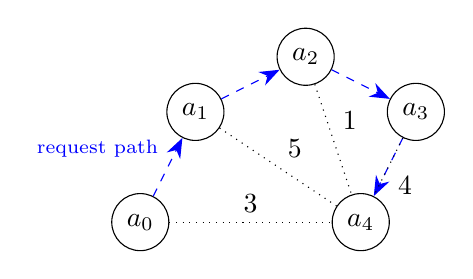
\begin{tikzpicture}
[bn/.style={circle,draw}
,root/.style={bn,thick}
,be/.style={dashed,draw=blue,arrows={-Stealth[scale=1.5]}}
,req/.style={bn,red!70!black}
,auto,scale=0.7]
\node[bn] (n1) at (0,0) {$a_{0}$};
\node[bn] (n2) at (1,2) {$a_{1}$};
\node[bn] (n3) at (3,3) {$a_{2}$};
\node[bn] (n4) at (5,2) {$a_{3}$};
\node[bn] (n5) at (4,0) {$a_{4}$};
\draw[be] (n1) -- node[blue]{\scriptsize{request path}} (n2);
\draw[be] (n2) -- (n3);
\draw[be] (n3) -- (n4);
\draw[be] (n4) -- (n5);
\draw[dotted] (n1) -- node{$3$} (n5);
\draw[dotted] (n2) -- node{$5$} (n5);
\draw[dotted] (n3) -- node{$1$} (n5);
\draw[dotted] (n4) -- node{$4$} (n5);
\end{tikzpicture}
\caption{The request arrives at $a_{4}$ which now needs to decide which one of $a_{0},\dots,a_{3}$ to choose as a new parent. For this it can access the edge costs to all of them.}
\end{subfigure}
\quad
\begin{subfigure}[t]{0.5\textwidth}
\centering
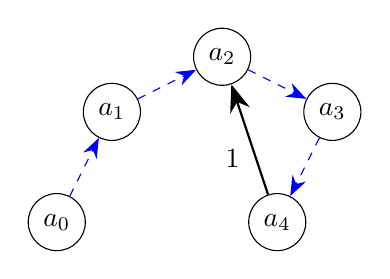
\begin{tikzpicture}
[bn/.style={circle,draw}
,root/.style={bn,thick}
,be/.style={dashed,draw=blue,arrows={-Stealth[scale=1.5]}}
,req/.style={bn,red!70!black}
,auto,scale=0.7]
\node[bn] (n1) at (0,0) {$a_{0}$};
\node[bn] (n2) at (1,2) {$a_{1}$};
\node[bn] (n3) at (3,3) {$a_{2}$};
\node[bn] (n4) at (5,2) {$a_{3}$};
\node[bn] (n5) at (4,0) {$a_{4}$};
\draw[be] (n1) -- (n2);
\draw[be] (n2) -- (n3);
\draw[be] (n3) -- (n4);
\draw[be] (n4) -- (n5);
\draw[thick,arrows={-Stealth[scale=1.5]}] (n5) -- node{$1$} (n3);
\end{tikzpicture}
\caption{$a_{2}$ gets chosen as the new parent since the edge towards it has the smallest cost.}
\end{subfigure}
\caption{Edge Cost Minimizer example with four node in the request path.}
\label{fig:ecm}
\end{figure}

\section{Local Pair Distance Minimizer}\label{alg:lpm}

An even better measure to minimize is the total distance between all pairs of nodes in the spanning tree $T$, defined as
\begin{equation}
\mathcal{C}_{pairs}(T) = \sum_{u,v\in V, u\neq v}c_T(u,v)
\end{equation}

where $c_T(u,v)$ is the cost of the shortest path between nodes $u$ and $v$ in the tree. Tree mutations aside, this directly corresponds to the performance of Arvy algorithms with uniformly random requests, since all pairs of nodes have the same probability of being used, meaning their distance in the tree contributes the same amount to the cost of an average request. In \autoref{tree:mpd} we discuss such minimal trees further. Notably the complexity to calculate this optimal tree is $\mathcal{O}(n^n)$, so unrealistic for many nodes. In addition, nodes don't have access to a global view of the graph at runtime which is needed to calculate the minimum pair distance tree.

We can however devise a heuristic that minimizes pair distance in a local subgraph consisting of only the nodes in the request path. Specifically when node $a_{k+1}$ needs to select a new parent node out of the candidates $A_k=\{a_{0},\dots,a_{k}\}$, it looks at the tree graph $T=(A_k,E')$ (with $E'\subset A_k\times A_k$) of nodes in the request path that was constructed from the parent selections of all previous nodes in the path. It then selects the node $a_{i}$ such that selecting this node yields the lowest possible pair distance, meaning $\mathcal{C}_{pairs}(T_i)$ with $T_i=(A_k\cup a_{k+1},E'\cup(a_{i},a_{k+1}))$ is minimal. See \autoref{fig:lpm} for an example.

\begin{algorithmic}
\Function{SelectNewParent}{$A_k$}
\State\Return$a_{i}$ such that $\mathcal{C}_{pairs}(T_i)$ is minimal, use highest $i$ for tie-breaking
\EndFunction
\end{algorithmic}

\begin{figure}[H]
\begin{subfigure}[t]{0.5\textwidth}
\centering
\begin{tikzpicture}[arvy-expl,scale=2,font=\scriptsize]
\node[v] (0) at (0,0) {$a_{0}$};
\node[v] (1) at (0,2) {$a_{1}$};
\node[v] (2) at (2,3) {$a_{2}$};
\draw[e] (1) --node[left]{4} (0);
\draw[dashed] (2) --node[below=2pt]{6} (0);
\draw[e] (2) --node[above]{5} (1);
\end{tikzpicture}
\caption{$a_{2}$ chooses $a_{1}$ as its new parent, since the total pair distance for that tree $\mathcal{C}_{pairs}(T_1)=c_{T_1}(a_{0},a_{1})+c_{T_1}(a_{0},a_{2})+c_{T_1}(a_{1},a_{2})=4+9+5=18$ is smaller than the one for $a_{0}$ which would be $4+10+6=20$}
\end{subfigure}
\quad
\begin{subfigure}[t]{0.5\textwidth}
\centering
\begin{tikzpicture}[arvy-expl,scale=2,font=\scriptsize]
\node[v] (0) at (0,0) {$a_{0}$};
\node[v] (1) at (0,2) {$a_{1}$};
\node[v] (2) at (2,3) {$a_{2}$};
\node[v] (3) at (3,1) {$a_{3}$};
\draw[e] (1) --node[left]{4} (0);
\draw[dashed] (2) --node[below=2pt]{6} (0);
\draw[e] (2) --node[above]{5} (1);
\draw[dashed] (0) --node[below]{2} (3);
\draw[e] (3) --node[above]{3} (1);
\draw[dashed] (2) --node[right]{2} (3);
\end{tikzpicture}
\caption{Even though edge $(a_{3},a_{1})$ has the highest cost, $a_{3}$ chooses $a_{1}$ as its new parent, since it minimizes the total pair distance. Here $\mathcal{C}_{pairs}(T_0)=37$, $\mathcal{C}_{pairs}(T_1)=36$, $\mathcal{C}_{pairs}(T_2)=38$}
\end{subfigure}
\caption{Local Pair Distance Minimizer example}
\label{fig:lpm}
\end{figure}

\section{Recursive Clique}
\label{alg:reclique}

As we'll see in \autoref{result:clique}, Ivy performs well on cliques of less than 5 nodes. 
Taking advantage of this fact, we design a graph resembling a clique, but where each node can contain another clique within, and so on. See \autoref{fig:reclique} for an example with 2 levels of cliques and each level having a clique of 3 nodes. This resulting recursive clique graph allows running Ivy recursively, taking advantage of Ivy's performance in each recursion level, scaling to many more nodes.

\begin{figure}[H]
\centering
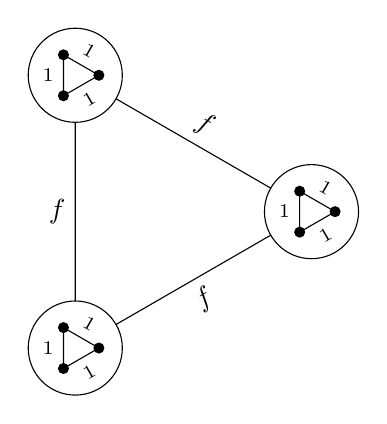
\begin{tikzpicture}
\coordinate (A) at (0:2);
\path (A) +(0:0.3) coordinate (AA);
\path (A) +(120:0.3) coordinate (AB);
\path (A) +(240:0.3) coordinate (AC);
\coordinate (B) at (120:2);
\path (B) +(0:0.3) coordinate (BA);
\path (B) +(120:0.3) coordinate (BB);
\path (B) +(240:0.3) coordinate (BC);
\coordinate (C) at (240:2);
\path (C) +(0:0.3) coordinate (CA);
\path (C) +(120:0.3) coordinate (CB);
\path (C) +(240:0.3) coordinate (CC);

\draw (A) -- node[above,sloped]{$f$} (B) -- node[left]{$f$} (C) -- node[below,sloped]{$f$} (A);

\fill[white] (A) circle [radius=17pt];
\fill[white] (B) circle [radius=17pt];
\fill[white] (C) circle [radius=17pt];
\draw (A) circle [radius=17pt];
\draw (B) circle [radius=17pt];
\draw (C) circle [radius=17pt];

\foreach \x in {A,B,C}
  \foreach \y in {A,B,C}
    \fill (\x\y) circle [radius=2pt];

\draw (AA) -- node[above,sloped]{\scriptsize{1}} (AB) -- node[left]{\scriptsize{1}} (AC) -- node[below,sloped]{\scriptsize{1}} (AA);
\draw (BA) -- node[above,sloped]{\scriptsize{1}} (BB) -- node[left]{\scriptsize{1}} (BC) -- node[below,sloped]{\scriptsize{1}} (BA);
\draw (CA) -- node[above,sloped]{\scriptsize{1}} (CB) -- node[left]{\scriptsize{1}} (CC) -- node[below,sloped]{\scriptsize{1}} (CA);

\end{tikzpicture}
\caption{Recursive Clique graph with $l=2$ levels and $b=3$ nodes in each level. Nodes in the same lowest level clique have distance $1$ between them, while nodes in different lowest level cliques have distance $f$ between them. Three virtual nodes group together three non-virtual nodes each}
\label{fig:reclique}
\end{figure}

A recursive clique graph has a level count parameter $l$ representing the number of levels and a base parameter $b$ for the number of nodes in a clique on a single level. We call the nodes in all levels except the lowest one \textit{virtual}, because they only exist to group non-virtual nodes in lower levels together. The total number of nodes in such a graph is $b^l$. In addition, for defining costs between edges, we declare a parameter $f>1$ for the factor by which edge cost increases from a lower to a higher level. This factor represents how far apart nodes in higher levels are. We define nodes in a clique in the lowest level to have distance $1$ from each other. For arbitrary nodes we can define the cost as

\begin{equation}
c(u,v)=\begin{cases}
0 & \text{if $u=v$} \\
1 & \text{otherwise if $u$ and $v$ share the same lowest level} \\
f & \text{otherwise if $u$ and $v$ share the same second-lowest level} \\
f^2 & \text{otherwise if $u$ and $v$ share the same third-lowest level} \\
\vdots & \\
f^{l-1} & \text{otherwise, $u$ and $v$ are in different nodes of the highest level} \\
\end{cases}
\end{equation}

When running a recursive Ivy algorithm on such a graph, the guiding rules are:
\begin{enumerate}
\item\label{reclique-invariant} The spanning tree needs to maintain the invariant that only at most one connection between all virtual nodes on a single level can exist. This ensures that if a request was made from within the virtual node where the token currently is at, the request path does not exit that virtual node. In addition this means there a request path can include at most $b-1$ edges of length $f^{l-1}$ from the most upper level (and similarly for lower levels), therefore limiting the number of long edges.
\label{reclique-rule-conn}
\item Connect to the earliest possible node in the request path. This ensures that the inverted arrows on the request path lead future requests to the root on the fastest way possible while still satisfying rule \ref{reclique-rule-conn}. This gives Ivy-like shortcut behavior on each level and across levels.
\label{reclique-rule-early}
\end{enumerate}

See \autoref{fig:reclique-alg} for an example of how this algorithm behaves with these rules. Note that this algorithm is specialized to graphs with these specific costs. In order to potentially have good performance with this algorithm on arbitrary graph costs an algorithm for finding the best clique level assignment/clustering needs to be run.

While in this heuristic we only limit ourselves to these three parameters for simplicity, this idea can be extended much further: Each level can contain arbitrary graphs and costs. As an example, with three nodes at the top-most level, the first node could contain a subgraph of a star, the second node a ring graph and the third node yet another nested graph. This then also calls for running different Arvy heuristics on each level, using whichever works best for that levels graph, making this a very flexible approach. In a realistic scenario, the top-most level can represent different data centers around the world, the level below different racks in the data center and the level below that different machines in a rack.

\begin{figure}[H]
\begin{subfigure}[t]{0.5\textwidth}
\centering
\begin{tikzpicture}
[be/.style={draw=black,arrows={-Stealth[scale=1.5]}}]
\coordinate (A) at (0:1.8);
\path (A) +(0:0.5) coordinate (AA);
\path (A) +(120:0.5) coordinate (AB);
\path (A) +(240:0.5) coordinate (AC);
\coordinate (B) at (120:1.8);
\path (B) +(0:0.5) coordinate (BA);
\path (B) +(120:0.5) coordinate (BB);
\path (B) +(240:0.5) coordinate (BC);
\coordinate (C) at (240:1.8);
\path (C) +(0:0.5) coordinate (CA);
\path (C) +(120:0.5) coordinate (CB);
\path (C) +(240:0.5) coordinate (CC);

\draw[be] (AB) -- (AA);
\draw[be] (AC) -- (AA);
\draw[be] (BB) -- (BA);
\draw[be] (BC) -- (BA);
\draw[be] (CB) -- (CA);
\draw[be] (CC) -- (CA);
\draw[be] (BA) to[out=0,in=90] (AA);
\draw[be] (CA) to[out=0,in=-90] (AA);

\foreach \x in {A,B,C}
  \foreach \y in {A,B,C}
    \fill (\x\y) circle [radius=2pt];

\fill[green!70!black] (AA) circle [radius=2pt,green];

\fill[red] (CC) circle [radius=2pt,fill=red];
\node[below=0 of CC] {\scriptsize{$a_{0}$}};
\node[below right=0 and -5pt of CA] {\scriptsize{$a_{1}$}};
\node[right=0 of AA] {\scriptsize{$a_{2}$}};

\end{tikzpicture}
\caption{The tree we start with satisfies the \hyperref[reclique-invariant]{tree invariant}, since between all three virtual nodes there is only at most one connection. The first node $a_{0}$ on the request path makes a request for the token which lies at root node $a_{2}$. $a_{2}$ will invert its arrow to point to $a_{0}$ with a long edge, which the invariant allows because the previous long edge $(a_{1},a_{2})$ is discarded when the request traverses it}
\label{fig:reclique-alg-a}
\end{subfigure}
\quad
\begin{subfigure}[t]{0.5\textwidth}
\centering
\begin{tikzpicture}
[be/.style={draw=black,arrows={-Stealth[scale=1.5]}}]
\coordinate (A) at (0:1.8);
\path (A) +(0:0.5) coordinate (AA);
\path (A) +(120:0.5) coordinate (AB);
\path (A) +(240:0.5) coordinate (AC);
\coordinate (B) at (120:1.8);
\path (B) +(0:0.5) coordinate (BA);
\path (B) +(120:0.5) coordinate (BB);
\path (B) +(240:0.5) coordinate (BC);
\coordinate (C) at (240:1.8);
\path (C) +(0:0.5) coordinate (CA);
\path (C) +(120:0.5) coordinate (CB);
\path (C) +(240:0.5) coordinate (CC);

\draw[be] (AB) -- (AA);
\draw[be] (AC) -- (AA);
\draw[be] (BB) -- (BA);
\draw[be] (BC) -- (BA);
\draw[be] (CB) -- (CA);
\draw[be] (CA) -- (CC);
\draw[be] (BA) to[out=0,in=90] (AA);
\draw[be] (AA) to[out=-90,in=-20] (CC);

\foreach \x in {A,B,C}
  \foreach \y in {A,B,C}
    \fill (\x\y) circle [radius=2pt];

\fill[green!70!black] (CC) circle [radius=2pt,green];

\fill[red] (CB) circle [radius=2pt,fill=red];
\node[above=0 of CB] {\scriptsize{$a_{0}$}};
\node[right=0 of CA] {\scriptsize{$a_{1}$}};
\node[left=0 of CC] {\scriptsize{$a_{2}$}};

\end{tikzpicture}
\caption{In the new tree, $a_{0}$ makes a request for the token at $a_{2}$ in the same virtual node. As with normal Ivy, all nodes will connect back to the node $a_{0}$ who made the original request. Notice that since the request was made from the same virtual node where the token currently resides, the virtual node wasn't exited and no long edge was traversed}
\end{subfigure}
\end{figure}

\begin{figure}
\ContinuedFloat
\begin{subfigure}[t]{0.5\textwidth}
\centering
\begin{tikzpicture}
[be/.style={draw=black,arrows={-Stealth[scale=1.5]}}]
\coordinate (A) at (0:1.8);
\path (A) +(0:0.5) coordinate (AA);
\path (A) +(120:0.5) coordinate (AB);
\path (A) +(240:0.5) coordinate (AC);
\coordinate (B) at (120:1.8);
\path (B) +(0:0.5) coordinate (BA);
\path (B) +(120:0.5) coordinate (BB);
\path (B) +(240:0.5) coordinate (BC);
\coordinate (C) at (240:1.8);
\path (C) +(0:0.5) coordinate (CA);
\path (C) +(120:0.5) coordinate (CB);
\path (C) +(240:0.5) coordinate (CC);

\draw[be] (AB) -- (AA);
\draw[be] (AC) -- (AA);
\draw[be] (BB) -- (BA);
\draw[be] (BC) -- (BA);
\draw[be] (CA) -- (CB);
\draw[be] (CC) -- (CB);
\draw[be] (BA) to[out=0,in=90] (AA);
\draw[be] (AA) to[out=-90,in=-20] (CC);

\foreach \x in {A,B,C}
  \foreach \y in {A,B,C}
    \fill (\x\y) circle [radius=2pt];

\fill[green!70!black] (CB) circle [radius=2pt,green];

\fill[red] (BB) circle [radius=2pt,fill=red];
\node[above=0 of BB] {\scriptsize{$a_{0}$}};
\node[above right=0 and -3pt of BA] {\scriptsize{$a_{1}$}};
\node[right=0 of AA] {\scriptsize{$a_{2}$}};
\node[below left=0 and -3pt of CC] {\scriptsize{$a_{3}$}};
\node[above=0 of CB] {\scriptsize{$a_{4}$}};

\end{tikzpicture}
\caption{The request path has two long edges, invoking the Ivy behavior on the upper level: $a_{3}$ will create a shortcut connection back to $a_{0}$. Then when $a_{4}$ receives the request, the rules disallow it from connecting back to $a_{0}$ as well, since this would lead to multiple edges between virtual nodes. Therefore $a_{4}$ has to connect back to $a_{3}$}
\end{subfigure}
\quad
\begin{subfigure}[t]{0.5\textwidth}
\centering
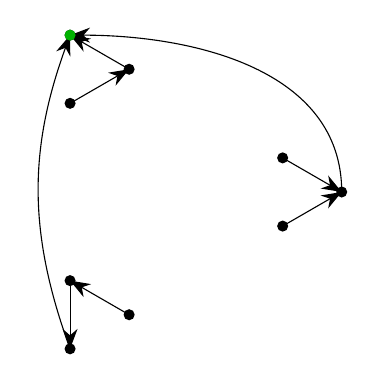
\begin{tikzpicture}
[be/.style={draw=black,arrows={-Stealth[scale=1.5]}}]
\coordinate (A) at (0:1.8);
\path (A) +(0:0.5) coordinate (AA);
\path (A) +(120:0.5) coordinate (AB);
\path (A) +(240:0.5) coordinate (AC);
\coordinate (B) at (120:1.8);
\path (B) +(0:0.5) coordinate (BA);
\path (B) +(120:0.5) coordinate (BB);
\path (B) +(240:0.5) coordinate (BC);
\coordinate (C) at (240:1.8);
\path (C) +(0:0.5) coordinate (CA);
\path (C) +(120:0.5) coordinate (CB);
\path (C) +(240:0.5) coordinate (CC);

\draw[be] (AB) -- (AA);
\draw[be] (AC) -- (AA);
\draw[be] (BA) -- (BB);
\draw[be] (BC) -- (BA);
\draw[be] (CA) -- (CB);
\draw[be] (CB) -- (CC);
\draw[be] (AA) to[out=90,in=0] (BB);
\draw[be] (CC) to[out=110,in=-110] (BB);

\foreach \x in {A,B,C}
  \foreach \y in {A,B,C}
    \fill (\x\y) circle [radius=2pt];

\fill[green!70!black] (BB) circle [radius=2pt,green];

\end{tikzpicture}
\caption{The resulting tree still only has $2$ long edges due to how the rules were enforced}
\end{subfigure}
\caption{Example of Recursive Clique heuristic on a recursive clique graph with parameters $l=2$ and $b=3$}
\label{fig:reclique-alg}
\end{figure}

\section{Fixed Ratio}

\paragraph{Hop-based}\label{alg:frh}

Another simple heuristic is one which chooses the node at a fixed ratio $0\leq f\leq 1$ between the first and the last one. As an example, with a request path $a_{0},a_{1},a_{2},a_{3},a_{4}$ and a ratio of $f=\frac{1}{2}$, node $a_{5}$ would choose $a_{2}$ as its new parent, since it's half-way between $a_{0}$ and $a_{4}$. We use the earlier node in case of a ratio being in-between two nodes. See \autoref{fig:fpr} for an example.

\begin{algorithmic}
\Function{SelectNewParent}{$A_k$}
\State\Return $a_{\lfloor f\cdot k\rfloor}$
\EndFunction
\end{algorithmic}

\begin{figure}[H]
\centering
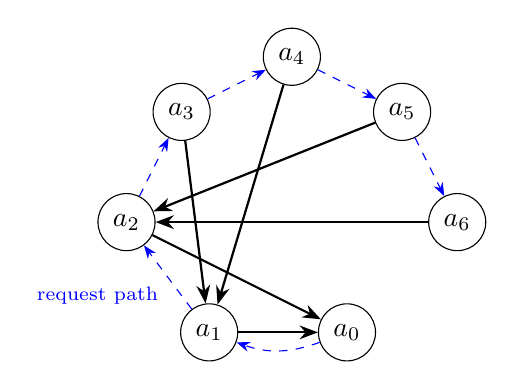
\begin{tikzpicture}
[bn/.style={circle,draw}
,root/.style={bn,thick}
,be/.style={thick,arrows={-Stealth[scale=1]}}
,pe/.style={dashed,draw=blue,arrows={-Stealth[scale=1]}}
,req/.style={bn,red!70!black}
,auto,scale=0.7]
\node[bn] (n0) at (4,0) {$a_{0}$};
\node[bn] (n1) at (1.5,0) {$a_{1}$};
\node[bn] (n2) at (0,2) {$a_{2}$};
\node[bn] (n3) at (1,4) {$a_{3}$};
\node[bn] (n4) at (3,5) {$a_{4}$};
\node[bn] (n5) at (5,4) {$a_{5}$};
\node[bn] (n6) at (6,2) {$a_{6}$};

\draw[pe] (n0) to[out=200,in=-20] (n1);
\draw[pe] (n1) -- node[blue]{\scriptsize{request path}} (n2);
\draw[pe] (n2) -- (n3);
\draw[pe] (n3) -- (n4);
\draw[pe] (n4) -- (n5);
\draw[pe] (n5) -- (n6);

\draw[be] (n1) -- (n0);
\draw[be] (n2) -- (n0);
\draw[be] (n3) -- (n1);
\draw[be] (n4) -- (n1);
\draw[be] (n5) -- (n2);
\draw[be] (n6) -- (n2);
\end{tikzpicture}
\caption{Hop-based Fixed Ratio heuristic with a ratio of $\frac{1}{2}$ and a request path of 7 nodes. Node $a_{6}$ chooses $a_{\lfloor \frac{1}{2}\cdot 5 \rfloor}=a_{2}$ as its parent. A binary tree is created as a result.}
\label{fig:fpr}
\end{figure}

\paragraph{Cost-based}\label{alg:frc}

A possible variation of this heuristic doesn't use the ratio on the node counts, but on the edge costs instead. A request path $A_k=\{a_{0},a_{1},a_{2},\dots,a_{k}\}$ gets mapped to costs $c_i$ representing how far the request had to travel to get to node $a_i$. Formally these costs are defined as
\begin{equation}
c_i=\sum_{j=1}^ic(a_{j-1},a_{j})
\end{equation}

The last node whose $c_i$ is lower than or equal to $f\cdot c_k$ is then selected.

\begin{algorithmic}
\Function{SelectNewParent}{$A_k$}
\State\Return $a_{i}$ with the maximum $i$ given the constraint $c_i\leq f\cdot c_k$ 
\EndFunction
\end{algorithmic}

These heuristics have the following interesting properties:
\begin{itemize}
\item For $f=0$ they are equivalent to Ivy. Similarly with $f=1$ they are equivalent to Arrow.
\item For $f=\frac{1}{m}, m\in\mathbb{N}$, the hop-based version builds a $m$-ary tree on the request path. See \autoref{fig:fpr} for an example of it building a binary tree with $m=2$.
\item If the costs are the same for all edges, the cost-based version is equivalent to the hop-based one.
\end{itemize}

\section{Dynamic Star}
\label{alg:dynstar}

To understand the Dynamic Star heuristic, we first look at the results from \cite{Peleg}, which for one is about finding a good tree to use for Arrow. A probability distribution $p_i, i\in V$ for each node making a request is given. Then the chance that a request travels from node $i$ to node $j$ is simply $p_ip_j$. Now let $d_T(i,j)$ be the cost to go from node $i$ to $j$ in some spanning tree $T$, similarly let $d_G(i,j)$ be the cost for the way from $i$ to $j$ by taking the shortest path in graph $G$. Then the expected cost of a single request in a tree and the graph respectively is
\begin{equation}
\begin{split}
c_R(T)\coloneqq & \sum_{i,j}p_ip_jd_T(i,j) \\
c_R(G)\coloneqq & \sum_{i,j}p_ip_jd_G(i,j) \\
\end{split}
\end{equation}

Now let $T_c$ denote a shortest-path tree from center node $c$, meaning a tree for which every node $v$ has a shortest path to $c$, i.e. $d_{T_c}(c,v)=d_G(c,v)$. The paper then shows that the $T_c$ with lowest $c_R(T_c)$ is a 2-approximation of the tree with lowest possible $c_R$:
\begin{equation}
c_R(T_c)\leq 2\cdot c_R(G)
\end{equation}

This means such a $T_c$ is a relatively good tree to use for Arrow, since the cost of the requests isn't much greater than the best possible path they could take. And since in our case we have a complete graph and metric costs, a shortest-path tree from node $c$ can simply be a star, connecting every other node to $c$ directly. With our complete graph weights $c:E\to\mathbb{N}^+$ this then reduces the calculation of $c_R(T_c)$ to
\begin{equation}
\label{dynstarc}
c_R(T_c)=\sum_{i,j}p_ip_j(c(i,c)+c(c,j))
\end{equation}

Now what this Dynamic Star heuristic does is it measures the distribution $p_i$ at runtime and dynamically adjusts the tree according to it, striving for a star. The fact that Arvy is a distributed algorithm however poses a problem, since nodes can't obtain a global view of the system to get accurate values for $p_i$, so we'll have to make do with every node $v$ having a local approximation $p_i^v$ of $p_i$.

To implement this the idea is that each node $v$ maintains counts $n_i^v\in\mathbb{N}_0$ of how many times each node $i$ made a request, initialized with all $0$. Because $v$ always knows how many requests it made itself, the value for $n_v^v$ is always accurate, while all others can be an outdated value. To update $n_i^v$ the following rules are used:
\begin{enumerate}
\item When node $v$ makes a request, set $n_v^v\gets n_v^v+1$
\label{rule1}
\item Any message sent from $v$ includes a subset of known counts $\{n_i^v,i\in S\subset V\}$, which when arriving at $u$ will update all received values if they are bigger than the values already known: $n_i^u\gets \max(n_i^u,n_i^v),i\in S$.
\end{enumerate}

Depending on the choice of the subset $S$ of value updates to send, the information propagation of the true values in the network might be slower or faster. Generally the bigger $|S|$, the faster information propagates. Here are some interesting choices for $S$:
\begin{itemize}
\item When node $v$ makes a request for the token, it only sends along its own request count with $S=\{v\}$, while all nodes along the request path use this same $S$. Since the only way for the rest of the network to know the accurate request count of the requesting node is for it to send the updated value, this is one of the most reasonable single-element choices for $S$ and is the choice that will be used for our simulations.
\item With every node forwarding all its values, we get $S=V$. Propagation of values is as fast as possible, but we also have $\mathcal{O}(n)$ complexity for the size of messages.
\item Message size can be reduced by making $S$ a uniform random selection of $V$, with $|S|\ll|V|$. With many requests happening, information should still propagate rather quickly.
\item An improved version of this is a random weighted selection, preferring $n_i^v$ that have been updated more recently.
\end{itemize}

Once such $n_i^v$ are known, the approximated request probabilities $p_i^v$ are then simply
\begin{equation}
p_i^v=\frac{n_i^v}{\sum_jn_j^v}
\end{equation}

With this we have everything in place for the heuristic to select a new parent out of the available options $A_k=\{a_{0},a_{1},\dots,a_k\}$. We do so by selecting the $a_{i}$ with the lowest cost as the center of the star.

\begin{algorithmic}
\Function{SelectNewParent}{$A_k$}
\State\Return Choose $a_{i}$ with lowest $c_R(T_{a_{i}})$, \\\qquad use highest $i$ for tie-breaking
\EndFunction
\end{algorithmic}

Justification is needed for the fact that the node $a_{k+1}$ selecting the new parent seems to access costs not imminent to it with the calculation of all $c_R(T_{a_{i}})$, which was given as a restriction in \hyperref[model]{the model}. This can be circumvented by each node $a_{i}$ calculating $c_R(T_{a_{i}})$ locally when the request travels through it, which is allowed since in \autoref{dynstarc} only accesses costs next the center node $a_{i}$ (this wouldn't be possible for non-star shortest path trees). Then that value can get sent in the message to all subsequent nodes in the request path, which can then use this result for the selection of the minimum. Note however that this is not exactly the same as calculating all $c_R(T_{a_{i}})$ values in the final node in the request path, since values for $n_i^v$ will be different, but it's the best we can do.

Unfortunately this algorithm needs $\mathcal{O}(n^2)$ time for the calculation of $c_R(T_{a_i})$ in each node along the request path, making it very slow to run in comparison to other algorithms. Messages need to send $S$ and the $a_{i}$ with lowest $c_R(T_{a_{i}})$ (as an optimization), resulting in $\mathcal{O}(|S|)$ message size.

\subsection{Non-converging Dynamic Star}

One slight problem with the Dynamic Star heuristic is that in general it eventually converges to a static tree. This is because as the total number of request increases, changes to $n_i^v$ matter less. After $R\in\mathbb{N}$ requests, another request can only cause a maximum change to $p_i^v$ of
\begin{equation}
\begin{split}
\left|p_i^v-p_i^{'v}\right| = & \left|\frac{n_i^v}{\sum_jn_j^v}-\frac{n_i^{'v}}{\sum_jn_j^{'v}}\right| = \left|\frac{n_i^v}{R}-\frac{n_i^v+\{0,1\}}{R+1}\right| \\
= & \left|\frac{n_i^vR+n_i^v-n_i^vR+\{0,1\}R}{R(R+1)}\right| = \frac{\left|n_i^v-\{0,1\}R\right|}{R(R+1)} \\
\leq & \frac{R}{R(R+1)}=\frac{1}{R+1}\to_{R\to\infty} 0
\end{split}
\end{equation}

where $\{0,1\}$ is $1$ or $0$ depending on whether $n_i^v$ was incremented or not.

This is a problem because it means the longer a system runs, the less it's adapting to changes in the probability pattern. If after $10^{100}$ requests a request-controlling adversary shows up, it could exploit this practically static tree by constantly bouncing requests between nodes with a slow connection. If this were to happen in the beginning, it wouldn't be a problem as the heuristic could adapt to this by choosing a better star center quickly. This means the algorithm's behavior is dependent on how long it has been running.

An idea to solve this problem is to give less weight to older requests, which can be done in multiple ways:
\begin{itemize}
\item After every increment of $n_i^v$ by one, all counts get decreased by a constant factor: $\forall i:n_i^v\gets \alpha\cdot n_i^v$ with $0<\alpha<1$. If this was a global view this would work well, since after $R$ requests an original contribution to $n_i^{global}$ of $1$ would be reduced to $\alpha^R$, implementing an exponential weight falloff. However since this isn't a global view, it won't work as well, because depending on the propagation speed with $|S|$, the $n_i^v$ will be more outdated, resulting in old requests having more weight than they would have in a global view.
\item A slight improvement over this can be achieved: For each message sent from $v$, the total amount of requests known $\sum_jn_j^v$ is sent along as well. When received by $u$, it's possible for it to calculate the difference of known requests $d\coloneqq\sum_jn_j^v-\sum_jn_j^u$. This means all $n_i^u$ are about that many requests more in the past than $n_i^v$, so an update is done on them to compensate for this: $\forall i:n_i^u\gets\alpha^d\cdot n_i^u$. This is better because the multiplication with $\alpha$ doesn't depend on the selection of $|S|$ anymore, resulting in older values being more accurately weighed.
\item With the requirement of nodes having a synchronized clock it's possible to improve on this: Every fixed time step, all counts in all nodes get decreased by the factor: $\forall i:n_i^v\gets \alpha\cdot n_i^v$. This is now an accurate time-based exponential falloff, independent of both the propagation speed and the request pattern.
\end{itemize}

This heuristic might work well in practice to guard against spontaneous adversaries, but for simplicity we will assume a uniform request pattern. Therefore we will not further evaluate this non-converging Dynamic Star heuristic.

\chapter{Graph Costs, Initial Trees and Request Sequences}

The performance of an Arvy algorithm depends not only on the algorithm itself, but also on the costs of the edges, the initial tree and the request sequence. In this section we describe all variations of these to be used in the simulations.

\section{Graph Costs}
\label{graph-costs}

\paragraph{Clique}\label{costs:clique} This is a cost function based on an underlying graph where all nodes are connected to each other with a unit cost.
\begin{equation}
c(u,v)=
\begin{cases}
0 & \text{if}\;u=v \\
1 & \text{otherwise}
\end{cases}
\end{equation}

%\paragraph{Ring} This cost function is based on a ring with unit costs as the underlying graph.
%\begin{equation}
%c(u,v)\equiv|u-v|\;(\bmod\;n)
%\end{equation}

\paragraph{Uniformly Random $d$-dimensional Hypercube}\label{costs:cube} These costs model uniformly random points $p_i:[0,1]^d$ in a $d$-dimensional hypercube, using the euclidean distance between them as the cost.
\begin{equation}
c(u,v)=\norm{p_u-p_v}_2
\end{equation}

\paragraph{Recursive Clique} These costs are given by the specialized graph of the Recursive Clique heuristic, see \autoref{alg:reclique}.

%\paragraph{Erdős-Rényi Random Graph} Generate a non-complete graph $G'$ by adding every possible edge independently with probability $p$. Then use that as the underlying graph with each edge having unit length.
%\begin{equation}
%c(u,v)=\text{length of shortest path from $u$ to $v$ in $G'$}
%\end{equation}
%
%\paragraph{Barabási-Albert Random Graph} For an $m\in\mathbb{N}$, start with a graph $G'=(\{1,\dots,m\},\varnothing)$. <- ??? Then iteratively add additional nodes while connecting it to $m$ existing nodes, with probabilities proportional to their degrees. This generates a scale-free network, where node degrees follow a power law, meaning only few nodes have high degree while many have low degree. The costs are then using this as an underlying graph. With $m=1$ this generates a tree as the underlying graph.

%\begin{equation}
%c(u,v)=\text{length of shortest path from $u$ to $v$ in $G'$}
%\end{equation}

\newpage
\section{Initial Trees}
\label{initial-trees}

\paragraph{Minimum Spanning Tree}\label{tree:mst}

The minimum spanning tree (MST) is the tree with lowest total edge cost. See \autoref{tree-examples} for an example of such a tree.

\paragraph{Uniformly Random Tree}\label{tree:random}

A uniformly random tree out of all possible trees. An algorithm for generating such a tree is as follows:

\begin{enumerate}
\item Select a random root node $r\gets_{u.a.r.}V$
\item Define $S=\{r\}$ to be the set of all nodes already included in the tree
\item Select a random node already in the tree $u\gets_{u.a.r.}S$
\label{random-tree-goto}
\item Select a random node not yet in the tree $v\gets_{u.a.r.}V\setminus S$
\item Output edge $(u,v)$ as part of the resulting tree
\item Set $S\gets S\cup\{v\}$
\item Unless $S=V$, go to \hyperref[random-tree-goto]{Step \ref{random-tree-goto}}
\end{enumerate}

\paragraph{Best Star Tree}\label{tree:star}

As we learned in \autoref{alg:dynstar}, the shortest-path tree with minimum $c_R(T_c)$ for some center node $c$ has at most two times longer paths than direct paths in the graph. By assuming uniformly random requests with $p_i=\frac{1}{n}$ for all nodes $i$, we can use this to generate an initial tree without knowing the request distribution. This also simplifies the calculation for $c_R(T_c)$ to
\begin{equation}
\begin{split}
c_R(T_c)&=\sum_{i,j}\frac{1}{n}\frac{1}{n}(c(i,c)+c(c,j))=\frac{1}{n^2}\sum_{i,j}c(i,c)+\frac{1}{n^2}\sum_{i,j}c(c,j) \\
&=\frac{n}{n^2}\sum_{i}c(i,c)+\frac{n}{n^2}\sum_{j}c(c,j)=\frac{2}{n}\sum_{i}c(i,c) \\
\end{split}
\end{equation}

This means finding $c_R(T_c)$ for a single $c$ can be done in time $\mathcal{O}(n)$ and for finding the best $c$ with smallest $c_R(T_c)$ only $\mathcal{O}(n^2)$ is needed. See \autoref{tree-examples} for an example of such a tree.

\paragraph{Minimum Pair Distance Tree}\label{tree:mpd}

This initial tree minimizes arguably most important measure for the Arrow algorithm: The average distance between all pairs of nodes. This is important because with uniformly random requests, every pair of nodes has the same chance of occurring subsequently in the request sequence. Consequently the average time to satisfy a request is the average distance between all pairs of nodes. See \autoref{tree-examples} for an example of a tree with these properties. Noticeable is that central nodes are forming and not all short edges are used.

A way to calculate this minimum is by brute force search through all possible trees. However because there are as much as $n^{n-2}$ possible trees~\cite{Borchardt} in a graph of $n$ nodes, this is not practical for more than a couple nodes. A listing of all possible trees can be obtained by the $n^{n-2}$ Prüfer~\cite{Prufer} sequences, for each of which the total pair distance needs to be found which is of order $\mathcal{O}(n^2)$ (with an algorithm similar to the one described in the next paragraph), giving a total complexity of $\mathcal{O}(n^n)$. \TODO{mention how this is different from low-stretch trees}


\paragraph{Approximated Minimum Pair Distance Tree}\label{tree:ampd}

Because calculating the actual minimum pair distance tree is impractical, we describe an algorithm that constructs a tree in $\mathcal{O}(n^3)$ time that tries to minimize total pair distance as well as possible. First let $c_T(u, v)$ denote the distance of the shortest path from $u$ to $v$ in a tree graph $T=(V',E')$ of nodes $V'\subset V$ and edges $E'\subset E$. Then let $\mathcal{C}_{pairs}(T)$ denote the total distance between all pairs of nodes in $T$.
\begin{equation}
\mathcal{C}_{pairs}(T) = \sum_{u,v\in V'}c_T(u,v)
\end{equation}

The algorithm is based on the idea of connecting nodes one-by-one to the tree, in every step choosing the node and a connecting edge that minimizes the total pair distance. We do this efficiently by maintaining a data structure that allows querying the increase of total pair distance for a node and edge in constant time.

Let $V'$ be the set of nodes currently included in the tree. $V'$ gets initialized to $\{r\}$ where $r$ is an arbitrarily chosen node. Our data structure then encompasses an array $p:V'\to\mathbb{R}$, where $p(v)$ stores the total distance from node $v$ to all other nodes in the current tree. In addition, a two-dimensional array $s:(V',V')\to\mathbb{R}$ is needed, where $s(u,v)$ stores the shortest distance in the tree between nodes $u$ and $v$.
\begin{equation}
\begin{split}
p(v)=&\sum_{i\in V'}c_T(i,v) \\
s(u,v)=&\;c_T(u,v)\\
\end{split}
\end{equation}

Now if node $v\in V\setminus V'$ and edge $(u,v)$ with $u\in V'$ were to get added to the tree to get $T'=T\cup(\{v\}, \{(u,v)\})$, the total pair distance increases only by the new pairs from $v$ to all nodes in $V'$. With our data structure we can calculate this increase in constant time:
\begin{equation}
\begin{split}
& \mathcal{C}_{pairs}(T')-\mathcal{C}_{pairs}(T) \\
=\;&\sum_{i\in V'}c_{T'}(i, v)+\sum_{i\in V'}c_{T'}(v, i)=2\sum_{i\in V'}c_{T'}(i, v) \\
=\;&2\sum_{i\in V'}\left(c_T(i,u)+c(u,v)\right)=2\left(\sum_{i\in V'}c_T(i,u)+|V'|\cdot c(u,v)\right) \\
=\;&2\left(p(u)+|V'|\cdot c(u,v)\right) \\
\end{split}
\end{equation}

Then after this new node $v$ and edge $(u,v)$ is added to the tree we need to update our data structure, which we can do in linear time:
\begin{itemize}
\item The total distance from $v$ to all other nodes $p(v)$ is just the total distance to all other nodes from $u$, plus the new edge once for every node: $p(v)\gets p(u)+|V'|\cdot c(u,v)$
\item For all other nodes, $p$ needs to be increased by the shortest path to $v$, which is just the shortest path to $u$ plus the cost of the edge $(u,v)$: $p(i)\gets p(i)+s(i,u)+c(u,v)$ for all $i\in V'$
\item Also the shortest path from all nodes to $v$ gets initialized to the shortest path to $u$ plus the cost of the edge $(u,v)$: $s(i,v)\gets s(i,u)+c(u,v)$ for all $i\in V'$
\item Similarly the shortest path from $v$ to all nodes: $s(v,i)\gets c(v,u)+s(u,i)$ for all $i\in V'$
\end{itemize}

As a result, our algorithm looks as follows:
\begin{enumerate}
\item Set $V'=\{r\}$ for an arbitrary node $r\in V$ and initialize the data structure with $p(r)=0$ and $s(r,r)=0$
\item Add the edge $(u,v)$ ($u\in V'$ and $v\in V\setminus V'$) which increases the total pair distance by the minimum to the resulting tree, by choosing the minimum value for $2\left(p(u)+|V'|\cdot c(u,v)\right)$ between all candidates
\label{approxStep}
\item Update $p$ and $s$ with the new node and edge
\item Unless $V'=V$, go to \hyperref[approxStep]{step \ref{approxStep}}
\end{enumerate}

Because the tree gets one more node in every iteration, the sequence of the number of edges between tree and non-tree nodes is $1n,2(n-1),3(n-2),\dots,(n-1)2,n1$. Every iteration therefore takes $\mathcal{O}(n^2)$ time to find the edge minimizing additional pair distance and another $\mathcal{O}(n)$ to update the data structure. The total complexity of this algorithm is therefore $\mathcal{O}(n\cdot(n^2+n))=\mathcal{O}(n^3)$. See \autoref{tree-examples} for an example of a tree constructed with this algorithm.

\begin{figure}
\centering
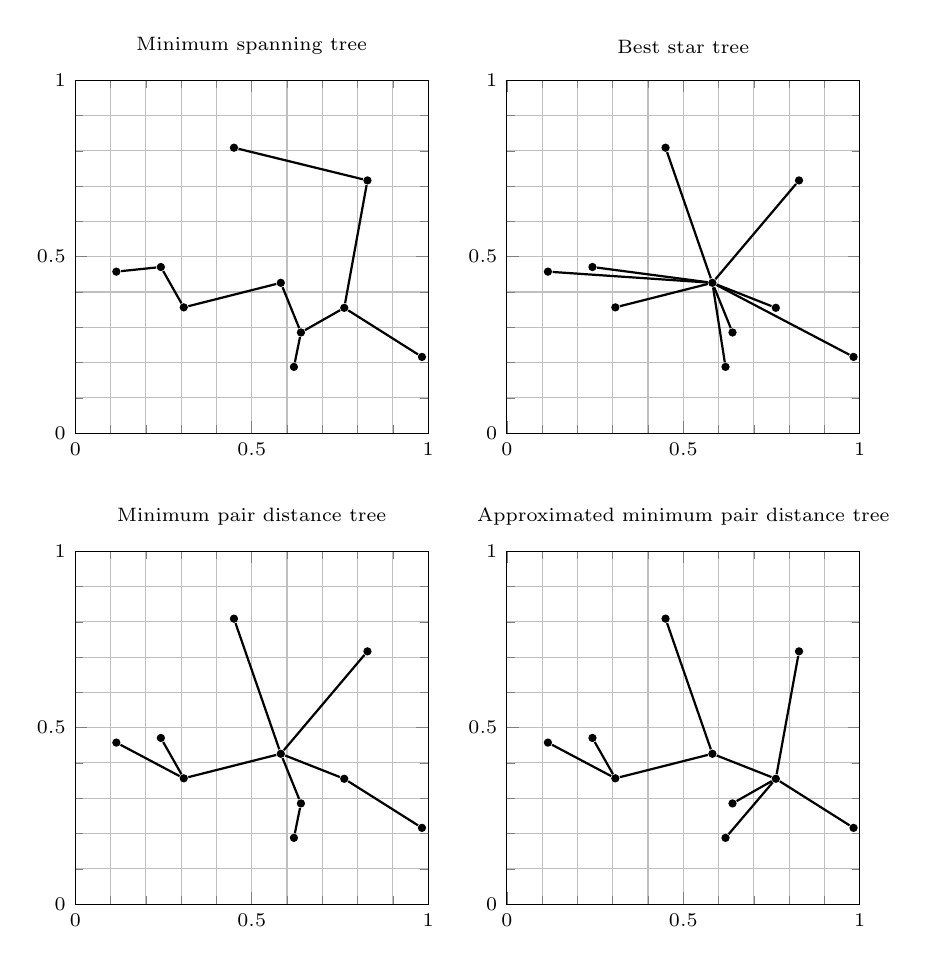
\begin{tikzpicture}[font=\scriptsize]
\begin{groupplot}[
  group style = {
    group size = 2 by 2,
    vertical sep = 1.5cm,
  },
  xtick distance = 0.5,
  ytick distance = 0.5,
  minor tick num = 4,
  grid = both,
  width=0.5\textwidth,
  height=0.5\textwidth,
  xmin = 0,
  ymin = 0,
  xmax = 1,
  ymax = 1,
]
% Branch shortestPairs, seed 9
\newcommand{\treenodes}{
\node[fill,circle,inner sep=0pt, minimum size=3pt] (0) at (axis cs:0.9824309197096475,0.21600824801462992) {};
\node[fill,circle,inner sep=0pt, minimum size=3pt] (1) at (axis cs:0.11630147561620086,0.4576546448862291) {};
\node[fill,circle,inner sep=0pt, minimum size=3pt] (2) at (axis cs:0.6196010239841514,0.18770539954142618) {};
\node[fill,circle,inner sep=0pt, minimum size=3pt] (3) at (axis cs:0.24250681611552394,0.47081365649116447) {};
\node[fill,circle,inner sep=0pt, minimum size=3pt] (4) at (axis cs:0.6394214211843541,0.28528957307777114) {};
\node[fill,circle,inner sep=0pt, minimum size=3pt] (5) at (axis cs:0.4496280158440922,0.8089357592613995) {};
\node[fill,circle,inner sep=0pt, minimum size=3pt] (6) at (axis cs:0.8279469953621574,0.7162195110010463) {};
\node[fill,circle,inner sep=0pt, minimum size=3pt] (7) at (axis cs:0.7622011483120192,0.35511162694708265) {};
\node[fill,circle,inner sep=0pt, minimum size=3pt] (8) at (axis cs:0.5823928330845394,0.4259817586877246) {};
\node[fill,circle,inner sep=0pt, minimum size=3pt] (9) at (axis cs:0.30737214539965896,0.35642649418227856) {};
}
\nextgroupplot[title=Minimum spanning tree]
\treenodes
\draw[thick] (1) -- (3);
\draw[thick] (2) -- (4);
\draw[thick] (3) -- (9);
\draw[thick] (4) -- (7);
\draw[thick] (5) -- (6);
\draw[thick] (6) -- (7);
\draw[thick] (7) -- (0);
\draw[thick] (8) -- (4);
\draw[thick] (9) -- (8);
\nextgroupplot[title=Best star tree]
\treenodes
\draw[thick] (0) -- (8);
\draw[thick] (1) -- (8);
\draw[thick] (2) -- (8);
\draw[thick] (3) -- (8);
\draw[thick] (4) -- (8);
\draw[thick] (5) -- (8);
\draw[thick] (6) -- (8);
\draw[thick] (7) -- (8);
\draw[thick] (9) -- (8);
\nextgroupplot[title=Minimum pair distance tree]
\treenodes
\draw[thick] (0) -- (7);
\draw[thick] (1) -- (9);
\draw[thick] (2) -- (4);
\draw[thick] (3) -- (9);
\draw[thick] (4) -- (8);
\draw[thick] (5) -- (8);
\draw[thick] (6) -- (8);
\draw[thick] (7) -- (8);
\draw[thick] (9) -- (8);
\nextgroupplot[title=Approximated minimum pair distance tree]
\treenodes
\draw[thick] (1) -- (9);
\draw[thick] (2) -- (7);
\draw[thick] (3) -- (9);
\draw[thick] (4) -- (7);
\draw[thick] (5) -- (8);
\draw[thick] (6) -- (7);
\draw[thick] (7) -- (0);
\draw[thick] (8) -- (7);
\draw[thick] (9) -- (8);
\end{groupplot}
\end{tikzpicture}
\caption{Different trees on a 10-node graph of uniformly random points in the unit square}
\label{tree-examples}
\end{figure}

\section{Request Sequences}
\label{request-sequences}

\paragraph{Uniformly Random Requests}\label{req:random} This request sequence distributes requests uniformly across all nodes, the request probability for each node $v$ is therefore $p_v=\frac{1}{n}$.

\paragraph{Adversarial Requests}\label{req:adversary} This request sequence represents an adversary that can control which nodes make requests while being able to inspect the current tree. For selecting a new request it selects the node furthest away by cost from the token in the current spanning tree.

\chapter{Implementation Notes}

As part of this thesis, a Haskell library for writing and testing Arvy heuristics was created, accessible at \url{https://github.com/infinisil/arvy}. In this chapter we explain some key design decisions that went into it. Most notably, Haskell's advanced type system allowed guaranteeing correctness of all Arvy heuristics defined with this library. We will look at parts of the file \href{https://github.com/Infinisil/arvy/blob/1bdac2aa8e599372f2b058d26ec9c33fd53d7a72/lib/Arvy/Algorithm.hs}{$\texttt{lib/Arvy/Algorithm.hs}$} where the core of this library is defined. Needless to say, this chapter is more technical than the others and advanced Haskell knowledge is required to fully understand it.

\section{Request Path abstraction}

An Arvy heuristic is correct if nodes can only set their new parent to nodes that were previously visited on the request path. With each node being referenced as an integer, this would be a problem, because a node $a_{k+1}$ could simply set $parent(a_{k+1})=0$ even though it might very well be the case that $0\notin A_k=\{a_{0},\dots,a_{k}\}$, which would be an invalid choice. So instead of representing nodes as integers, we represent them as some arbitrary type with certain capabilities that reflect it being part of the request path. In particular such types will not be constructible on their own.

One such trivial capability we'll need is that once we have some node index, we can forward that value via messages to other nodes. This makes sense to require, since some node $a_{k+1}$ can't know about the possible new parents $\{a_{0},\dots,a_{k}\}$ unless these nodes somehow forwarded their own indices along with the messages. In Haskell, this forwarding can be represented as a typeclass on two types $i_a$ and $i_b$, where $i_a$ represents a node index earlier in the request path than node index $i_b$. We will state that if you have a value of $i_a$ you can get a value of $i_b$, which can be done with a typeclass parametric on those types, holding a function for converting from $i_a$ to $i_b$. This typeclass is trivially implementable for all same types $i=i_a=i_b$, since forwarding will then simply be the identity function.

\begin{minted}{haskell}
-- | A class for node indices that can be forwarded between nodes
class Forwardable ia ib where
  forward :: ia -> ib

-- | All equivalent types can be trivially forwarded
instance Forwardable i i where
  forward = id
\end{minted}

Now we need to somehow encode a request path in a type. In such a request path the important constraint is that messages are only sent in one direction, meaning node indices can only be forwarded in one direction as well. Looking at it from the perspective of a single node in the request path, we can forward from its predecessor to the current node and from the current node to its successor. Encoding this as a typeclass leaves us with the following for representing a node (index).

\begin{minted}{haskell}
class ( Forwardable (Pred i) i
      , Forwardable i (Succ i)
      ) => NodeIndex i where
  -- The type representing the previous node
  type Pred i :: *
  -- The type representing the successor node
  type Succ i :: *
\end{minted}

Now of course defining different types for every node along the request path is impossible, we can only use this to prove correctness. So for the implementation, we can use normal integers to represent all nodes.

\begin{minted}{haskell}
type Node = Int

instance NodeIndex Node where
  -- Predecessors and successors in the request path are
  -- all nodes represented by integers as well
  type Pred Node = Node
  type Succ Node = Node
\end{minted}

\section{Arvy Heuristic Abstraction}

The most important part of defining an Arvy algorithm is the heuristic it uses to decide the new parent node. We extend this to the notion of a \textit{behavior}, which includes not only how new parents are selected, but also how it gets decided what a request message looks like, how the initial message is generated, and what the final node receiving the message does. Each node on the request path should be allowed to run arbitrary code.

For representing computations we use the relatively new effect library \href{https://hackage.haskell.org/package/polysemy}{Polysemy}. In this library a computation is described with the type $\texttt{Sem r a}$ where $\texttt{r}$ represents the possible effects it can have and $\texttt{a}$ being the result of the computation. As an example, a computation that's allow to use randomness and returns a boolean is described by the type $\texttt{Sem '[Random] Bool}$. With this said, the main type for defining an Arvy heuristic is defined as follows.

\begin{minted}{haskell}
{- |
An Arvy heuristic for a dynamic algorithm.
- @i@ is the node index type
- @msg :: * -> *@ is the type of request messages passed between
  nodes, parametrized by the node index type for allowing messages
  to forward node indices
- @r@ is the effects the algorithm runs in, which can include
  effects parametrized by @i@ in order to allow effects dependent
  on indices -}
data ArvyBehavior i msg r = ArvyBehavior
  { -- | What message the node making the request should send to
    -- its parent
    arvyMakeRequest
    :: i -- ^ The current node index
    -> Succ i -- ^ The index of the parent node
    -> Sem r (msg i) -- ^ Returns the message to send to the parent

  , -- | What parent an intermediate node should select when
    -- receiving a message, and what message to forward to its
    -- parent
    arvyForwardRequest
    :: msg (Pred i) -- ^ The received message
    -> i -- ^ The current node index
    -> Succ i -- ^ The parent node
    -> Sem r (Pred i, msg i) -- ^ The new parent to select and
                             -- the message to forward

  , -- | Called only for the last node in the request sequence
    -- that's holding the token
    arvyReceiveRequest
    :: msg (Pred i) -- ^ The received message
    -> i -- ^ The current node index
    -> Sem r (Pred i) -- ^ The new parent to select
  }
\end{minted}

This succinct-yet-complicated type includes a lot of information. As an overview, when a node makes a request for the token, $\texttt{arvyMakeRequest}$ is called, which generates a message to be sent to the nodes parent. Then when a message arrives at a node, depending on whether it has the token or not, the functions $\texttt{arvyReceiveRequest}$ or $\texttt{arvyForwardRequest}$ are called respectively, the latter of which then needs to generate another message for forwarding. Function $\texttt{arvyForwardRequest}$ is the most interesting one since it has to handle both receiving and sending a message, so we'll look more closely at its type signature.

For one it says that nodes receive messages of type $\texttt{msg (Pred i)}$ whose values can only include node indices of predecessors to the current node in the request path. It then needs to return a value of $\texttt{Pred i}$ as the new parent for the current node. With the way node indices are defined in the previous section, the only possible values to return are ones received from the message. This means to select a new parent, nodes have to decode the message which will contain node indices given by past nodes, then return one of them.

In addition, the function receives values $\texttt{i}$ and $\texttt{Succ i}$ representing the current node index and the current nodes parent respectively. In addition to the new parent node to select, the function also needs to return a $\texttt{msg i}$ representing the message to be forwarded. The $\texttt{msg}$ type being parametrized by $\texttt{i}$ enforces that this message can only contain node indices to previous nodes (since all previous node indices $\texttt{Pred i}$ can be forwarded to $\texttt{i}$) or the current node (which is of type $\texttt{i}$ already). $\texttt{Succ i}$ however can't be sent in the message because there's no way to convert it to type $\texttt{i}$.

Functions $\texttt{arvyMakeRequest}$ and $\texttt{arvyReceiveRequest}$ are special cases of $\texttt{arvyForwardRequest}$. The former is special in that a node making a request does not receive any message and it doesn't need to select a new parent since it becomes the root. The latter is special in that the final root node receiving the request doesn't have a parent and doesn't need to forward a message. Having separate functions for these greatly simplifies the code.

\chapter{Results}

In this chapter we simulate Arvy algorithms on different \textit{scenarios} to see how they perform. A scenario consists of these variations:
\begin{itemize}
\item Node count: The number of nodes in the graph, this is in the range 10 to 1000, depending on the execution speed.
\item Graph costs: The cost of all edges in the graph, see \autoref{graph-costs} for possible values. We focus on \hyperref[costs:cube]{uniformly random 2-dimensional hypercube} costs since it provides interesting and realistic values, even for a low number of nodes.
\item Request sequence: Which nodes get requests and how many of them, see \autoref{request-sequences} for possible values. The number of requests ranges from $10^5$ to $10^6$.
\end{itemize}

We then run different Arvy algorithms from \autoref{algs} with different initial trees on such scenarios and compare them against each other. Initial trees are described in \autoref{initial-trees}. Since all heuristics except Arrow change the tree structure, we run those with a uniformly random initial tree, such that this shouldn't have any influence on the execution. Only for Arrow itself we vary the initial tree to find the best one to use.

For evaluating how well heuristics perform we look at the measures defined in \autoref{model-perf}. This includes the average request time $\mathcal{C}_{time}$ and the average request hops $\mathcal{C}_{hops}$. In addition, to get a feeling for the evolution of the tree we sometimes look at the average tree edge distance in the spanning tree $T=(V',E')$ over time, defined as
\begin{equation}
\mathcal{C}_{edges}(T)=\frac{1}{|E'|}\sum_{(u,v)\in E'}c(u,v)
\end{equation}

\newcommand{\evalTime}{Average request time $\mathcal{C}_{time}$}
\newcommand{\evalHops}{Average request hops $\mathcal{C}_{hops}$}
\newcommand{\evalEdges}{Average tree edge distance $\mathcal{C}_{edges}$}

\pgfplotsset{
  every axis legend/.append style={
    at={(0.5,1.03)},
    anchor=south
  },
  legend cell align = left,
  legend image post style = {
    line width = 3pt,
  },
  width=0.9\textwidth,
  height=0.5\textwidth,
  legend columns = 3,
  every axis/.append style = {
    xmode = log,
    xmin = 1,
    grid,
    colormap name = colormap/jet,
    legend style = { font = \scriptsize },
    xlabel = Number of requests,
    no markers,
  },
  every axis plot post/.append style = {
    thick,
    x={x},
    line join=round,
  },
}

\newpage
\section{Best Initial Trees for Arrow}\label{result:trees}

For this evaluation we run Arrow on different initial trees to see how well they perform. We use only 10 nodes such that we can compute the \hyperref[tree:mpd]{minimum pair distance tree} in reasonable time. For graph costs we use uniformly random points from a 2-dimensional hypercube and we will use uniformly random requests. First we look at how the average time to satisfy requests changes over time:

\begin{tikzpicture}
\centering
\begin{axis}[
  ylabel = \evalTime,
  xmax = 100000,
  cycle list = { [samples of colormap=5] },
]
\pgfplotstableread{data/trees/time.dat}{\data}
\addplot table [y={arrow-random}] {\data};
\addlegendentry {Random tree}
\addplot table [y={arrow-mst}] {\data};
\addlegendentry {Minimum spanning tree}
\addplot table [y={arrow-shortpairs}] {\data};
\addlegendentry {Approx. min. pair dist. tree}
\addplot table [y={arrow-star}] {\data};
\addlegendentry {Best star tree}
\addplot table [y={arrow-shortestpairs}] {\data};
\addlegendentry {Min. pair dist. tree}
\end{axis}
\end{tikzpicture}

Not surprisingly, the tree minimizing pair distance outperforms every other tree. However due to its running time of $\mathcal{O}(n^n)$ it won't be very practical for more nodes. Interestingly the next best one is the best star tree with only a running time of $\mathcal{O}(n^2)$, followed closely by the approximated minimum pair distance tree with runtime $\mathcal{O}(n^3)$. The minimum spanning tree comes next with a slightly worse time. Understandably, a completely random tree is not a good tree to use for low average request time. Conclusively we will use the best star tree for future performance evaluations of Arrow on this scenario. Now let's also look at the number of hops for each of them:

\begin{tikzpicture}
\centering
\begin{axis}[
  ylabel = \evalHops,
  xmax = 100000,
  cycle list = { [samples of colormap=5] },
]
\pgfplotstableread{data/trees/hops.dat}{\data}
\addplot table [y={arrow-random}] {\data};
\addlegendentry {Random tree}
\addplot table [y={arrow-mst}] {\data};
\addlegendentry {Minimum spanning tree}
\addplot table [y={arrow-shortpairs}] {\data};
\addlegendentry {Approx. min. pair dist. tree}
\addplot table [y={arrow-star}] {\data};
\addlegendentry {Best star tree}
\addplot table [y={arrow-shortestpairs}] {\data};
\addlegendentry {Min. pair dist. tree}
\end{axis}
\end{tikzpicture}

As one would expect from trees it has a very low hop count. This value is lower than $2$ because nodes can make requests when they have the token already, giving a hop count of $0$, and the center node always has a hop count $\leq 1$. Interestingly the random tree tree has a decently low hop count.

Note that while this is only the result for a single random seed with only 10 nodes, the results are similar for other configurations. Also since in this case the tree never changes, it would be possible to calculate accurate expectations for these measures without having to rely on a simulation.

\section{Tree Convergence}\label{result:convergence}

In this section we look at the behavior of heuristics in regards to the tree they end up with after many uniformly random requests. To get a feeling for the tree evolution we look at the trees average tree edge cost. We use only $100$ nodes since the Dynamic Star heuristic is quite slow to run. For edge costs we use uniformly random points in a 2-dimensional hypercube. In addition to looking at the average tree edge cost, we also plot some fixed baselines for known trees. This includes one for the minimum spanning tree, one for the best star tree, and one for a uniformly random tree. All algorithms start with an initially completely random tree.

\begin{tikzpicture}
\centering
\begin{axis}[
  ylabel = \evalEdges,
  xmax = 100000,
  cycle list = { [samples of colormap=8] },
]
\pgfplotstableread{data/converging/treeWeight.dat}{\data}
\addplot table [y={arrow-random}] {\data};
\addlegendentry {Uniformly random tree}
\addplot table [y={arrow-star}] {\data};
\addlegendentry {Best star tree}
\addplot table [y={arrow-mst}] {\data};
\addlegendentry {Min. sp. tree}
\addplot table [y={random-random}] {\data};
\addlegendentry {Random}
\addplot table [y={ivy-random}] {\data};
\addlegendentry {Ivy}
\addplot table [y={dynamicStar-random}] {\data};
\addlegendentry {\hyperref[alg:dynstar]{Dynamic star}}
\addplot table [y={localMinPairs-random}] {\data};
\addlegendentry {\hyperref[alg:lpm]{Local pair dist. min.}}
\addplot table [y={minWeight-random}] {\data};
\addlegendentry {\hyperref[alg:ecm]{Edge cost min.}}
\end{axis}
\end{tikzpicture}

What we can see from this plot:
\begin{itemize}
\item The dynamic star heuristic converges to the best star tree, indicated by their lines merging into one. The fact that the line does not jitter in the end indicates a converged tree. This makes sense since they both optimize for a minimal $c_R(T_c)$ with a uniform request distribution. Only with very bad luck of a lot of requests to the same nodes in a row it is possible for it to stray from a best star tree, getting more improbable the longer it runs.
\item The edge cost minimizer heuristic as expected converges to the minimum spanning tree, as already predicted in \autoref{alg:ecm}. Here we can directly see how this algorithm only ever decreases tree edge costs, indicated by its line monotonically decreasing until it reaches the lowest possible state of the minimum spanning tree.
\item The Ivy algorithm seems to continuously have a tree with high edge costs, in the same range as a completely random tree. This makes more or less sense since Ivy does not look at edge costs at all when selecting new parent nodes. If we were to include the hop-based fixed ratio heuristic in this plot it would show the same result for the same reason. The same happens for the random heuristic in this plot.
\item Interestingly, the local pair distance minimizer heuristic seems to go towards a rather low average edge cost with no known baseline tree in that region.
\end{itemize}

From this we conclude that the eventual behavior of the dynamic star and edge cost minimizer heuristics can be achieved by simply using Arrow on the best star tree and the minimum spanning tree respectively. Therefore we don't further look at these heuristics.

\section{Fixed Ratio Heuristics}

Here we look at the fixed ratio class of algorithms, both hop-based and weight-based ones, with different values for the ratio $f$, including $f=0$ for Ivy and $f=1$ for Arrow, and steps of $\frac{1}{8}$ between them. We will be using 1000 nodes with uniformly random 2-dimensional hypercube costs and uniformly random requests. We will be using Arrow with the best star tree as a baseline. All fixed ratio algorithms will start with a completely random tree.

\begin{tikzpicture}
\centering
\begin{axis}[
  ylabel = \evalTime,
  xmax = 1000000,
  cycle list = { [samples of colormap=10] },
  legend columns = 5,
]
\pgfplotstableread{data/ratio/time.dat}{\data}
\addplot table [y={arrow-star}] {\data};
\addlegendentry {Best star Arrow}
\addplot table [y={inbetween-0-1-random}] {\data};
\addlegendentry {$f=\frac{0}{8}$ (Ivy)}
\addplot table [y={inbetween-1-8-random}] {\data};
\addlegendentry {$f=\frac{1}{8}$}
\addplot table [y={inbetween-1-4-random}] {\data};
\addlegendentry {$f=\frac{2}{8}$}
\addplot table [y={inbetween-3-8-random}] {\data};
\addlegendentry {$f=\frac{3}{8}$}
\addplot table [y={inbetween-1-2-random}] {\data};
\addlegendentry {$f=\frac{4}{8}$}
\addplot table [y={inbetween-5-8-random}] {\data};
\addlegendentry {$f=\frac{5}{8}$}
\addplot table [y={inbetween-3-4-random}] {\data};
\addlegendentry {$f=\frac{6}{8}$}
\addplot table [y={inbetween-7-8-random}] {\data};
\addlegendentry {$f=\frac{7}{8}$}
\addplot table [y={inbetween-1-1-random}] {\data};
\addlegendentry {$f=\frac{8}{8}$ (Arrow)}
\end{axis}
\end{tikzpicture}

From this we can see that generally, the lower the ratio, the lower average request time. This is somewhat explainable by seeing that with a lower ratio more shortcuts are created. However for some reason ratios around $f=\frac{6}{8}$ seem to converge to some average request time lower than all others. So mysteriously $f=\frac{6}{8}=\frac{3}{4}$ with the hop-based fixed ratio heuristic is not too bad of an algorithm to use for this scenario \TODO{explanation? Maybe look at this with different number of nodes, different graph weights}. We now also look at the weight-based fixed ratio heuristics:

\begin{tikzpicture}
\centering
\begin{axis}[
  ylabel = \evalTime,
  xmax = 100000,
  cycle list = { [samples of colormap=10] },
  legend columns = 5,
]
\pgfplotstableread{data/ratio2/time.dat}{\data}
\addplot table [y={arrow-star}] {\data};
\addlegendentry {Best star Arrow}
\addplot table [y={inbetween2-0.0-random}] {\data};
\addlegendentry {$f=\frac{0}{8}$ (Ivy)}
\addplot table [y={inbetween2-0.125-random}] {\data};
\addlegendentry {$f=\frac{1}{8}$}
\addplot table [y={inbetween2-0.25-random}] {\data};
\addlegendentry {$f=\frac{2}{8}$}
\addplot table [y={inbetween2-0.375-random}] {\data};
\addlegendentry {$f=\frac{3}{8}$}
\addplot table [y={inbetween2-0.5-random}] {\data};
\addlegendentry {$f=\frac{4}{8}$}
\addplot table [y={inbetween2-0.625-random}] {\data};
\addlegendentry {$f=\frac{5}{8}$}
\addplot table [y={inbetween2-0.75-random}] {\data};
\addlegendentry {$f=\frac{6}{8}$}
\addplot table [y={inbetween2-0.875-random}] {\data};
\addlegendentry {$f=\frac{7}{8}$}
\addplot table [y={inbetween2-1.0-random}] {\data};
\addlegendentry {$f=\frac{8}{8}$ (Arrow)}
\end{axis}
\end{tikzpicture}

With an initial look, the anomalies from the previous plot are not present anymore. However they now appear in the opposite direction: The ratios around $f=\frac{3}{4}$ are all \textit{above} the highest ratio, giving a performance ordering from best to worst of $\frac{0}{8}, \frac{1}{8}, \frac{2}{8}, \frac{3}{8}, \frac{8}{8}, \frac{4}{8}, \frac{5}{8}, \frac{6}{8}, \frac{7}{8}$. This is very peculiar and we can't explain the reason for this yet.

\section{Best Heuristics}\label{result:algs}

In this section we compare performances of different heuristics on uniformly random requests, ignoring the ones whose eventual behavior can be achieved with Arrow on a specific tree (this includes the \hyperref[alg:dynstar]{Dynamic Star} and \hyperref[alg:ecm]{Edge Cost Minimizer} heuristics). We will again be using uniformly random points in a 2-dimensional hypercube.

\begin{tikzpicture}
\centering
\begin{groupplot}[
  ylabel = \evalHops,
  xmax = 100000,
  cycle list = { [samples of colormap=4] },
  legend columns = 2,
  group style = {
    group size = 1 by 2,
    xlabels at = edge bottom,
    ylabels at = edge left,
  },
]
\nextgroupplot[ylabel=\evalTime]
\pgfplotstableread{data/algs/time.dat}{\data}
\addplot table [y={arrow-star}] {\data};
\addlegendentry {Best star Arrow}
\addplot table [y={ivy-random}] {\data};
\addlegendentry {Ivy}
\addplot table [y={localMinPairs-random}] {\data};
\addlegendentry {\hyperref[alg:lpm]{Local Pair Dist. Min.}}
\addplot table [y={inbetween-3-4-random}] {\data};
\addlegendentry {\hyperref[alg:frh]{Hop-based fixed ratio} with $f=\frac{3}{4}$}

\nextgroupplot[ylabel=\evalHops]
\pgfplotstableread{data/algs/hops.dat}{\data}
\addplot table [y={arrow-star}] {\data};
\addplot table [y={ivy-random}] {\data};
\addplot table [y={localMinPairs-random}] {\data};
\addplot table [y={inbetween-3-4-random}] {\data};
\end{groupplot}
\end{tikzpicture}

We can see that Arrow has better performance than all other heuristics, although both the local pair distance minimizer and hop-based fixed ratio heuristics get close to it. Since we used the best star tree with Arrow, it also beats others in the number of hops needed per request. The mysterious \hyperref[alg:frh]{Hop-based Fixed Ratio} heuristic ends up only slightly worse than Arrow after a number of requests. Regarding Ivy, even though it constructs a local star on the request path, it doesn't do nearly as well as a global star in Arrow, but at least it's better than the local pair distance minimizer heuristic which seems to lack in regards to hop count, contrary to its time-based performance.

\section{Adversarial requests}

In this section we look at the performance of heuristics for \hyperref[req:adversary]{adversarial requests}. Here we include the \hyperref[alg:dynstar]{dynamic star} heuristic again, since it only converges to the best star tree if requests are uniformly random and therefore doesn't show the same behavior as Arrow with that as a starting tree. Our scenario is 1000 nodes with costs of uniformly random points in a 2-dimensional hypercube.

\begin{tikzpicture}
\centering
\begin{groupplot}[
  xmax = 1000000,
  cycle list = { [samples of colormap=5] },
  legend columns = 2,
  group style = {
    group size = 1 by 2,
    xlabels at = edge bottom,
    ylabels at = edge left,
  },
]
\nextgroupplot[ylabel=\evalTime]
\pgfplotstableread{data/adversary/time.dat}{\data}
\addplot table [y={arrow-star}] {\data};
\addlegendentry {Best star Arrow}
\addplot table [y={ivy-random}] {\data};
\addlegendentry {Ivy}
\addplot table [y={localMinPairs-random}] {\data};
\addlegendentry {\hyperref[alg:lpm]{Local pair dist. min.}}
\addplot table [y={inbetween-3-4-random}] {\data};
\addlegendentry {\hyperref[alg:frh]{Hop-based fixed ratio} with $f=\frac{3}{4}$}
\addplot table [y={dynamicStar-random}] {\data};
\addlegendentry {\hyperref[alg:dynstar]{Dynamic star}}

\nextgroupplot[ylabel=\evalHops]
\pgfplotstableread{data/adversary/hops.dat}{\data}
\addplot table [y={arrow-star}] {\data};
\addplot table [y={ivy-random}] {\data};
\addplot table [y={localMinPairs-random}] {\data};
\addplot table [y={inbetween-3-4-random}] {\data};
\addplot table [y={dynamicStar-random}] {\data};
\end{groupplot}
\end{tikzpicture}

In this adversarial request case, the dynamic star heuristic seems to win out as the only heuristic that adapts its behavior based on request probabilities. Apparently it can go towards tree that doesn't allow such adversarial exploitation. Amazingly the fixed ratio algorithm is second place, followed by the local pair distance minimizer heuristic, which performs not too bad even with a high hop count. Perhaps by surprise, Ivy is the worst algorithm in this ranking.

\section{Ivy in Small Cliques}
\label{result:clique}

The fact that Arrow with the best star tree seems to have been the best heuristic on uniformly random requests so far gives the impression that perhaps Arrow can't be beaten at all. In this section we construct a counterexample by looking at Ivy in a clique with a low number of nodes. We use 3,4,5 and 6 nodes with clique graph costs. We compare Ivy with Arrow on the \hyperref[tree:mpd]{minimum pair distance tree}.

\begin{tikzpicture}
\begin{groupplot}[
  ylabel = \evalTime,
  xmax = 100000,
  cycle list = { [samples of colormap=2] },
  small,
  group style = {
    group size = 2 by 2,
    xlabels at = edge bottom,
    ylabels at = edge left,
    vertical sep = 1.5cm,
  },
]
\nextgroupplot[title={$3$ nodes},legend to name={CommonLegend1}]
\pgfplotstableread{data/low3/time.dat}{\3}
\addplot table [y={ivy-shortestpairs}] {\3};
\addlegendentry{Ivy}
\addplot table [y={arrow-shortestpairs}] {\3};
\addlegendentry{Arrow}

\nextgroupplot[title={$4$ nodes}]
\pgfplotstableread{data/low4/time.dat}{\4}
\addplot table [y={ivy-shortestpairs}] {\4};
\addplot table [y={arrow-shortestpairs}] {\4};

\nextgroupplot[title={$5$ nodes}]
\pgfplotstableread{data/low5/time.dat}{\5}
\addplot table [y={ivy-shortestpairs}] {\5};
\addplot table [y={arrow-shortestpairs}] {\5};

\nextgroupplot[title={$6$ nodes}]
\pgfplotstableread{data/low6/time.dat}{\6}
\addplot table [y={ivy-shortestpairs}] {\6};
\addplot table [y={arrow-shortestpairs}] {\6};

\end{groupplot}
\path[text=black] (group c1r1.north east) -- node[above=0.8cm]{\ref{CommonLegend1}} (group c2r1.north west);
\end{tikzpicture}

Here we can see that Ivy is in fact better than Arrow in this scenario with 3 or 4 nodes, but not with 5 (very closely) or 6 nodes. This pattern continues into higher node counts, Arrow beating Ivy for more than 5 nodes. The worse performance for higher node counts is explainable with what we've discovered in \autoref{result:convergence}: Ivy maintains a pretty random tree throughout, which as we've seen in \autoref{result:algs} leads to rather poor performance in comparison to Arrow. It is perhaps surprising that this doesn't hold for node counts of 3 and 4. For 3 nodes this is however easy to see since all requests paths with two hops in Ivy mean that the next request is guaranteed to be satisfied in one hop due to the shortcut behavior. With Arrow however this is not the case because all two-hop request paths can be followed by another two-hop request path in the other direction, since the tree structure is maintained. This beneficial short-cutting effect of Ivy seems to outweigh the tree randomization for 4 nodes as well, which makes sense since the number of trees is so low that they can't be randomized much.

\section{Recursive Clique}

In this section we will measure the performance of the \hyperref[alg:reclique]{recursive clique} heuristic with the hopes of it being the best heuristic to use for the type of graph it was made for. We use the parameters $l=6$, $b=3$ and $f=5$, meaning 6 levels of 3-node cliques for a total of $l^b=6^3=729$ nodes, with a cost of $f^{l-1}=5^{6-1}=3125$ between nodes in the highest level clique. We will use uniformly random requests.

We compare the performance to the usual heuristics of best star Arrow, \hyperref[alg:lpm]{local pair minimizer}, \hyperref[alg:frh]{hop-based fixed ratio} and Ivy. However we will add another contestant, namely Arrow starting with a minimum spanning tree. This is because a minimum spanning tree on such a recursive clique graph directly corresponds to a tree satisfying the \hyperref[reclique-invariant]{invariant} needed for recursive cliques heuristic, meaning there can be at most one edge between virtual nodes on the same layer, which is also beneficial to Arrow for the same reason it's beneficial to the recursive clique heuristic.

We first look at the average request time:

\begin{tikzpicture}
\begin{groupplot}[
  ylabel = \evalTime,
  xmax = 1000000,
  cycle list = { [samples of colormap=6] },
  small,
  group style = {
    group size = 2 by 1,
    xlabels at = edge bottom,
    ylabels at = edge left,
  },
]
\pgfplotstableread{data/reclique/time.dat}{\data}
\nextgroupplot[legend to name={CommonLegend}]
\addplot table [y={reclique}] {\data};
\addlegendentry {\hyperref[alg:reclique]{Recursive clique}}
\addplot table [y={arrow-star}] {\data};
\addlegendentry {Best star Arrow}
\addplot table [y={inbetween-3-4-random}] {\data};
\addlegendentry {\hyperref[alg:frh]{Hop-based Fixed Ratio} with $f=\frac{3}{4}$}
\addplot table [y={ivy-random}] {\data};
\addlegendentry {Ivy}
\addplot table [y={arrow-mst}] {\data};
\addlegendentry {Min. sp. tree Arrow}
\addplot table [y={localMinPairs-random}] {\data};
\addlegendentry {\hyperref[alg:lpm]{Local pair minimizer}}
\node (t) at (axis cs:1000000,2.4) {};
\node (b) at (axis cs:1000000,1.5) {};
\draw[thick,red,dashed] (axis cs:100000,2.4) rectangle (axis cs:1000000,1.5);

\nextgroupplot[xmin=100000,ymin=1.5,ymax=2.4]
\addplot table [y={reclique}] {\data};
\addplot table [y={arrow-star}] {\data};
\addplot table [y={inbetween-3-4-random}] {\data};
\addplot table [y={arrow-mst}] {\data};
\addplot table [y={localMinPairs-random}] {\data};
\end{groupplot}
\path[text=black] (group c1r1.north east) -- node[above=5pt]{\ref{CommonLegend}} (group c2r1.north west);
\draw[red,thick,dashed] (t) -- (group c2r1.north west);
\draw[red,thick,dashed] (b) -- (group c2r1.south west);
\end{tikzpicture}

Sure enough, the recursive clique heuristic wins over all others. The beneficial shortcut behavior of Ivy in 3-cliques is unsurprisingly maintained with multiple levels of cliques. We can also see that in this case Arrow with a minimum spanning tree does indeed perform better than Arrow on the best star tree. Ivy is the worst heuristic in this scenario, which makes sense as a random tree will have plenty of long edges. The mysterious fixed ratio heuristic maintains its decent performance as well. The local pair minimizer heuristic seems to converge towards the performance of a minimum spanning tree. We now also look at the average request hops for these heuristics:

\begin{tikzpicture}
\begin{axis}[
  ylabel = \evalHops,
  xmax = 1000000,
  cycle list = { [samples of colormap=6] },
]
\pgfplotstableread{data/reclique/hops.dat}{\data}
\addplot table [y={reclique}] {\data};
\addlegendentry {\hyperref[alg:reclique]{Recursive clique}}
\addplot table [y={arrow-star}] {\data};
\addlegendentry {Best star Arrow}
\addplot table [y={inbetween-3-4-random}] {\data};
\addlegendentry {\hyperref[alg:frh]{Hop-based Fixed Ratio} with $f=\frac{3}{4}$}
\addplot table [y={ivy-random}] {\data};
\addlegendentry {Ivy}
\addplot table [y={arrow-mst}] {\data};
\addlegendentry {Min. sp. tree Arrow}
\addplot table [y={localMinPairs-random}] {\data};
\addlegendentry {\hyperref[alg:lpm]{Local pair minimizer}}
\end{axis}
\end{tikzpicture}

What stands out in this plot is the fact that the fixed ratio heuristic seems to converge towards an average hop count of 2, which is the range of a star tree. We further look at the average tree edge distance:

\begin{tikzpicture}
\begin{axis}[
  ylabel = \evalEdges,
  xmax = 1000000,
  cycle list = { [samples of colormap=6] },
]
\pgfplotstableread{data/reclique/treeWeight.dat}{\data}
\addplot+[dashed,shorten <=3] table [y={reclique}] {\data};
\addlegendentry {\hyperref[alg:reclique]{Recursive clique}}
\addplot table [y={arrow-star}] {\data};
\addlegendentry {Best star Arrow}
\addplot table [y={inbetween-3-4-random}] {\data};
\addlegendentry {\hyperref[alg:frh]{Hop-based Fixed Ratio} with $f=\frac{3}{4}$}
\addplot table [y={ivy-random}] {\data};
\addlegendentry {Ivy}
\addplot+[dashed] table [y={arrow-mst}] {\data};
\addlegendentry {Min. sp. tree Arrow}
\addplot table [y={localMinPairs-random}] {\data};
\addlegendentry {\hyperref[alg:lpm]{Local pair minimizer}}
\end{axis}
\end{tikzpicture}

From this we can hypothesize that the local pair minimizer heuristic seems to converge towards a tree satisfying the \hyperref[reclique-invariant]{recursive clique tree invariant} as the minimum spanning tree already does as well. This would explain why it performs this well for $\mathcal{C}_{time}$.

\chapter{Summary}

\bibliographystyle{IEEEtran}
\bibliography{references}

\end{document}
